% Chapter 5: Testing and Evaluation
\chapter{Testing and Evaluation}
\label{ch:testing}

This chapter presents the testing strategy, functional test results, security
verification, route-optimisation evaluation, AI evaluation, and a mapping of
results against the fourteen project objectives defined in
Section~\ref{sec:objectives}.  All testing was performed by a single developer
using a physical Android device (Samsung Galaxy A54, Android~14) and the Chrome
desktop browser, reflecting the realistic constraints of an academic project.

% ─────────────────────────────────────────────────────────────
\section{Testing Strategy}
\label{sec:test-strategy}

Testing was organised into four tiers:

\begin{enumerate}
  \item \textbf{Unit tests}: automated Dart tests targeting the
        \texttt{TaskViewModel} business logic (task loading, offline queuing,
        sync recovery).
  \item \textbf{Functional tests}: manual end-to-end walkthroughs of every
        user-facing feature, recorded in Table~\ref{tab:func-admin} (admin)
        and Table~\ref{tab:func-driver} (driver).
  \item \textbf{Security tests}: cross-tenant Row-Level Security (RLS)
        verification and RBAC enforcement.
  \item \textbf{Quantitative evaluation}: route-optimisation distance
        measurements, AI response-quality assessment, and driver-recommendation
        accuracy.
\end{enumerate}

\noindent Figure~\ref{fig:test-pyramid} visualises how these four tiers build
upon one another, with the broadest automated coverage at the base narrowing
towards the quantitative evaluation at the apex.

\begin{figure}[H]
  \centering
  \resizebox{0.82\textwidth}{!}{%
  \begin{tikzpicture}[
      >=Stealth,
      every node/.style={font=\sffamily},
      layer/.style={
        trapezium, trapezium angle=75,
        draw=blue!40, thick, rounded corners=2pt,
        text=black, minimum height=1cm,
        trapezium stretches body,
        align=center
      }
    ]
    % Layers from bottom (widest) to top (narrowest)
    \node[layer, fill=blue!18, minimum width=12cm]
      (unit) {Unit Tests\\[-2pt]{\scriptsize Dart/Flutter \textbullet{} TaskViewModel \textbullet{} Automated}};
    \node[layer, fill=blue!14, minimum width=9cm, above=4pt of unit]
      (func) {Functional Tests\\[-2pt]{\scriptsize End-to-End Walkthroughs \textbullet{} Manual}};
    \node[layer, fill=blue!10, minimum width=6cm, above=4pt of func]
      (sec)  {Security Tests\\[-2pt]{\scriptsize RLS \textbullet{} RBAC \textbullet{} Cross-Tenant}};
    \node[layer, fill=blue!6, minimum width=3.5cm, above=4pt of sec]
      (quant){Quantitative Evaluation\\[-2pt]{\scriptsize Distance \textbullet{} AI Quality \textbullet{} Accuracy}};

    % Side annotations
    \draw[<->, thick, blue!50] ([xshift=-7mm]unit.south west)
      -- node[left, rotate=90, anchor=south, font=\sffamily\small, blue!70]
         {Increasing Specificity} ([xshift=-7mm]quant.north west);
    \draw[<->, thick, blue!50] ([xshift=7mm]unit.south east)
      -- node[right, rotate=-90, anchor=south, font=\sffamily\small, blue!70]
         {Increasing Automation} ([xshift=7mm]quant.north east);
  \end{tikzpicture}%
  }%
  \caption{Testing strategy pyramid: four tiers from broad automated
           unit coverage to focused quantitative evaluation.}
  \label{fig:test-pyramid}
\end{figure}

% ─────────────────────────────────────────────────────────────
\section{Unit Tests}
\label{sec:unit-tests}

Two automated unit tests validate the \texttt{TaskViewModel} using a
\texttt{\_FakeTaskRepository} that wraps an in-memory Drift database:

\begin{enumerate}
  \item \textbf{loadTasks}: seeds the repository, calls
        \texttt{viewModel.loadTasks()}, and asserts that the task list is
        non-empty and \texttt{isOffline} is \texttt{false}.
  \item \textbf{markAsDelivered (offline queue)}: configures the fake
        repository to simulate offline mode, marks a task as delivered with a
        proof code, asserts that \texttt{isOffline} becomes \texttt{true} and
        \texttt{pendingSyncCount} increments, then calls
        \texttt{syncPendingDeliveries()} and verifies the count returns to
        zero.
\end{enumerate}

\noindent Both tests pass under \texttt{flutter test} on the project CI
pipeline.

% ─────────────────────────────────────────────────────────────
\section{Functional Testing: Admin Portal}
\label{sec:func-admin}

Table~\ref{tab:func-admin} lists the admin-side functional test cases.  Each
test was executed manually through the Chrome web interface and verified
against the expected outcome.

\begin{longtable}{c p{3.4cm} p{4.2cm} c c}
  \caption{Admin portal functional test cases.}
  \label{tab:func-admin} \\
  \toprule
  \textbf{ID} & \textbf{Test Case} & \textbf{Expected Result} & \textbf{Pass} & \textbf{Fig.} \\
  \midrule
  \endfirsthead
  \toprule
  \textbf{ID} & \textbf{Test Case} & \textbf{Expected Result} & \textbf{Pass} & \textbf{Fig.} \\
  \midrule
  \endhead
  \midrule
  \multicolumn{5}{r}{\footnotesize\itshape Continued on next page} \\
  \endfoot
  \bottomrule
  \endlastfoot

  A1 & Login with admin credentials
     & Dashboard displayed with task list and navigation
     & \checkmark
     & \ref{fig:ss-a1} \\

  A2 & Create a new task (manual entry)
     & Task appears in list with status \emph{pending}
     & \checkmark
     & \ref{fig:ss-a2} \\

  A3 & Import tasks via CSV upload
     & All valid rows created; malformed rows rejected with error message
     & \checkmark
     & \ref{fig:ss-a3} \\

  A4 & Edit an existing task
     & Changes saved; updated fields visible on refresh
     & \checkmark
     & \ref{fig:ss-a4} \\

  A5 & Delete a task
     & Task removed from list; database row deleted
     & \checkmark
     & \ref{fig:ss-a5} \\

  A6 & Generate route (nearest-neighbour)
     & Route created with sequenced stops; map preview displayed
     & \checkmark
     & \ref{fig:ss-a6} \\

  A7 & View driver recommendation scores
     & Drivers ranked by composite score; availability, distance, and performance shown
     & \checkmark
     & \ref{fig:ss-a7} \\

  A8 & Fleet-wide optimisation
     & Tasks assigned to nearest available drivers; assignments table shown
     & \checkmark
     & \ref{fig:ss-a8} \\

  A9 & Review proof-of-delivery photo
     & PoD image and metadata displayed in review panel
     & \checkmark
     & \ref{fig:ss-a9} \\

  A10 & Send chat message to driver
      & Message appears in driver's chat; read receipt tracked
      & \checkmark
      & \ref{fig:ss-a10} \\

  A11 & Send broadcast message
      & All drivers in company receive the message
      & \checkmark
      & \ref{fig:ss-a11} \\

  A12 & AI summary (admin view)
      & Natural-language summary of fleet status displayed
      & \checkmark
      & \ref{fig:ss-a12} \\

  A13 & Customer tracking lookup (valid code)
      & Delivery status card displayed with address, driver, and PoD flag
      & \checkmark
      & --- \\

  A14 & Customer tracking lookup (invalid code)
      & Inline warning ``No delivery found'' displayed
      & \checkmark
      & --- \\
\end{longtable}

% ── Screenshot placeholders — Admin ──

\begin{figure}[H]
  \centering
  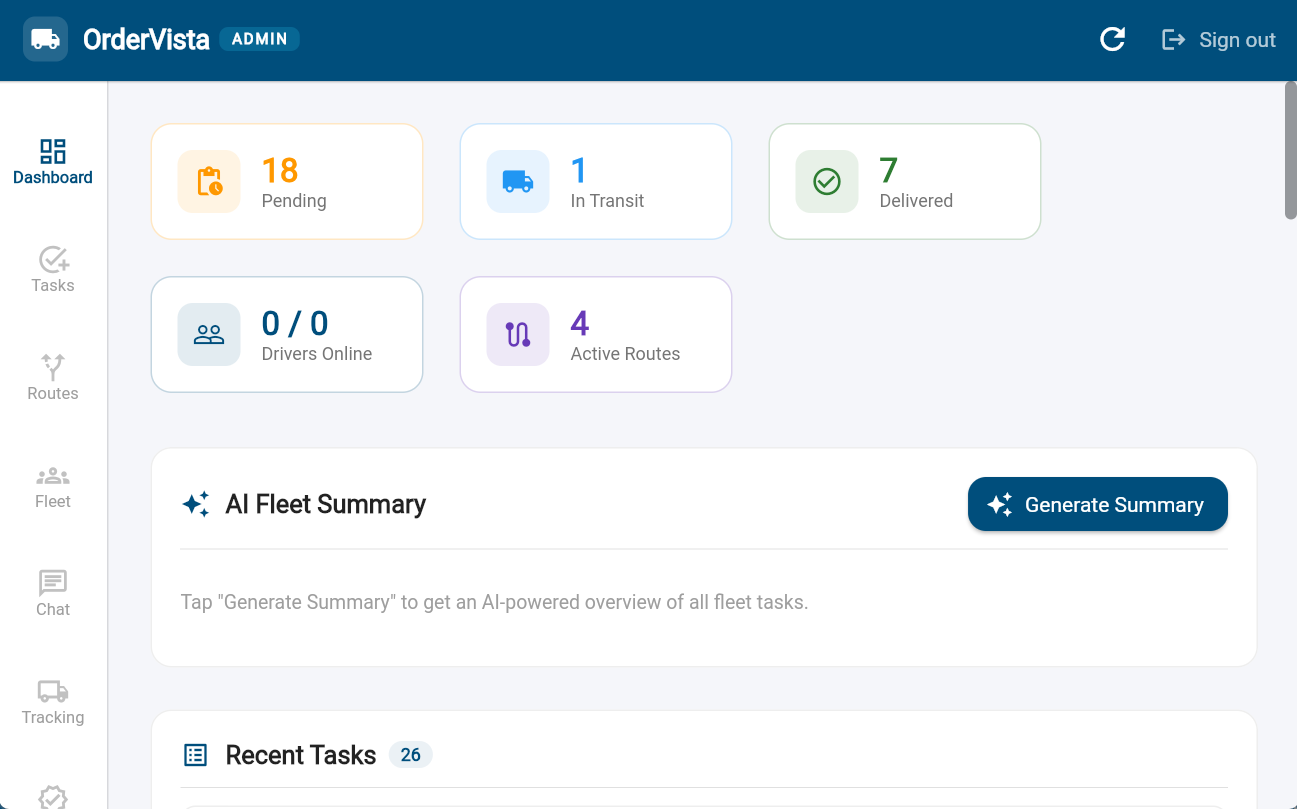
\includegraphics[width=0.7\textwidth]{ss-a1}
  \caption{Admin dashboard after login (A1).}
  \label{fig:ss-a1}
\end{figure}

\begin{figure}[H]
  \centering
  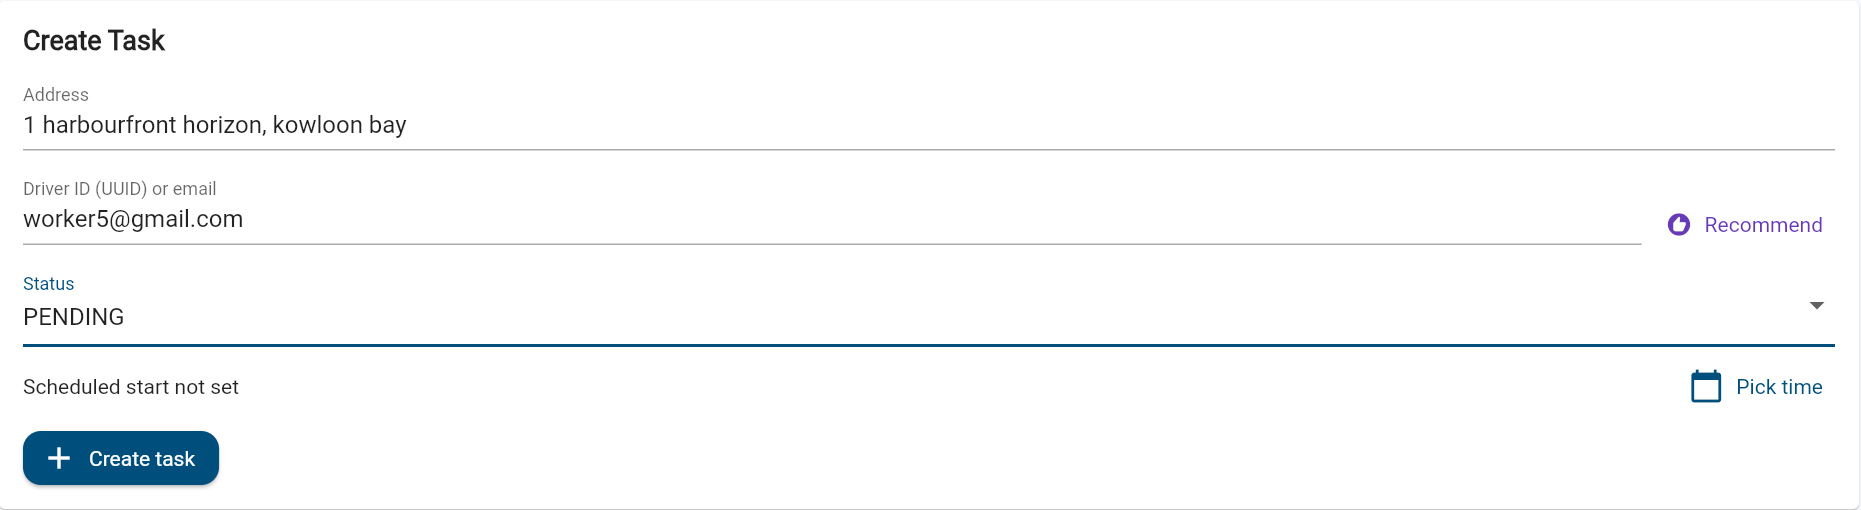
\includegraphics[width=0.7\textwidth]{ss-a2}
  \caption{Manual task creation form (A2).}
  \label{fig:ss-a2}
\end{figure}

\begin{figure}[H]
  \centering
  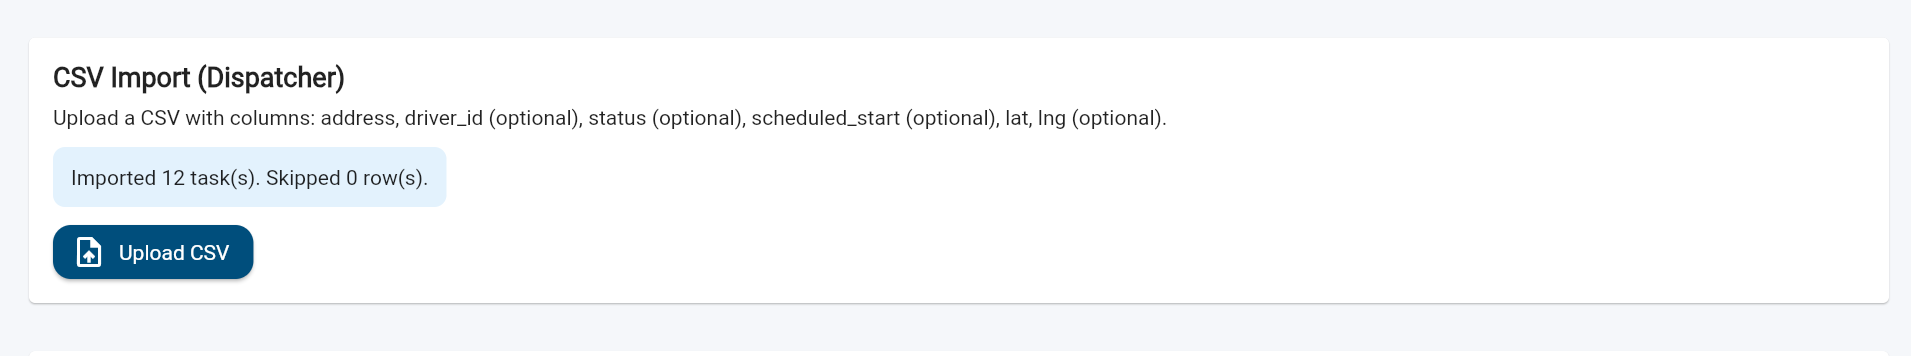
\includegraphics[width=0.7\textwidth]{ss-a3}
  \caption{CSV bulk import with error feedback (A3).}
  \label{fig:ss-a3}
\end{figure}

\begin{figure}[H]
  \centering
  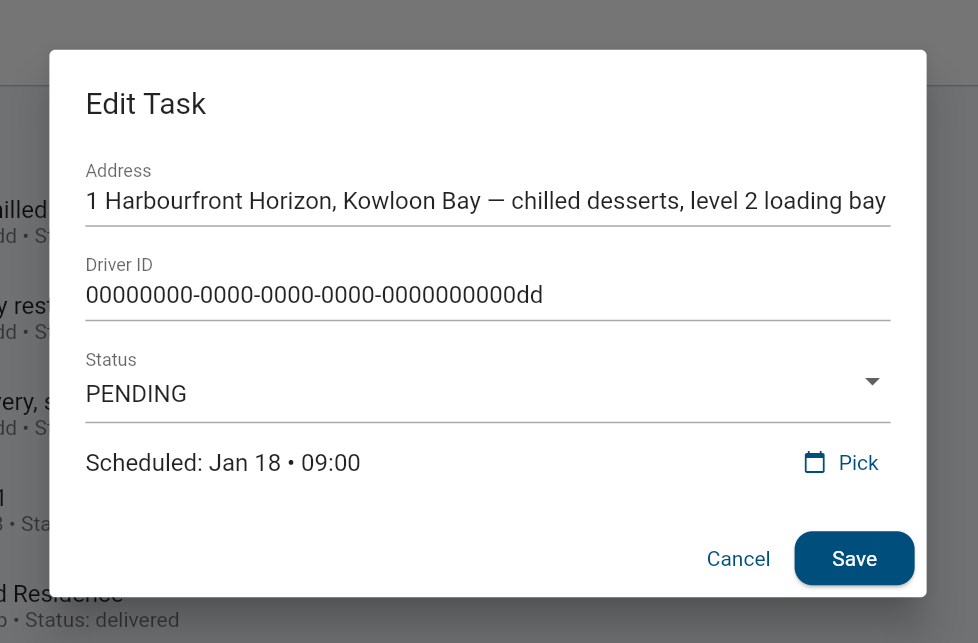
\includegraphics[width=0.7\textwidth]{ss-a4}
  \caption{Editing an existing task (A4).}
  \label{fig:ss-a4}
\end{figure}

\begin{figure}[H]
  \centering
  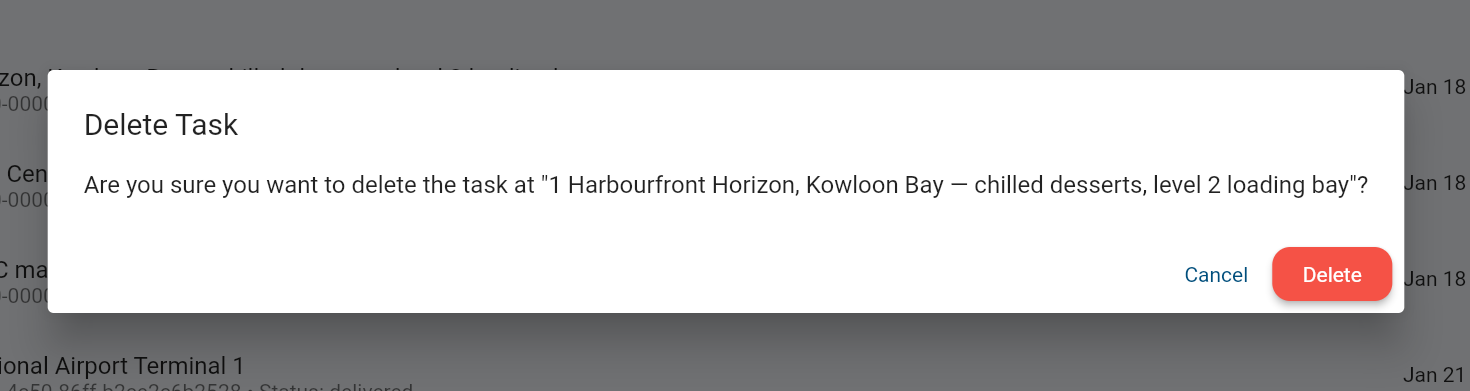
\includegraphics[width=0.7\textwidth]{ss-a5}
  \caption{Task deletion confirmation (A5).}
  \label{fig:ss-a5}
\end{figure}

\begin{figure}[H]
  \centering
  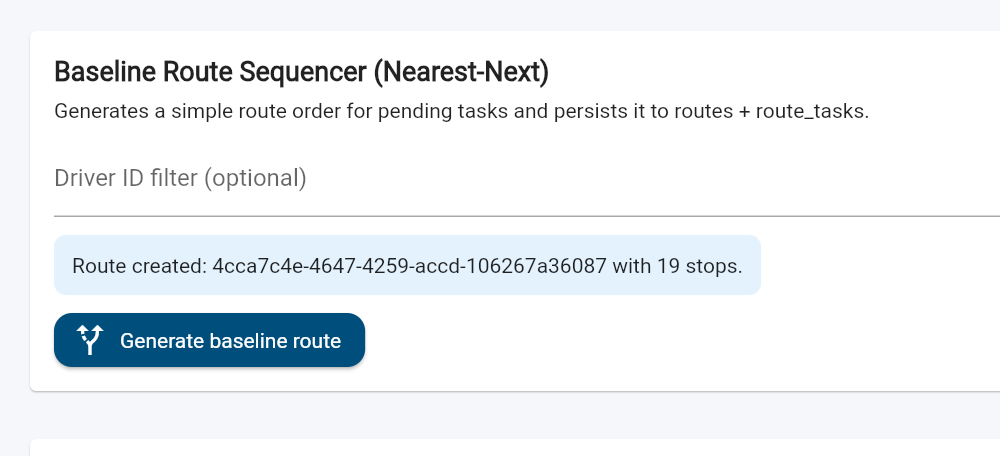
\includegraphics[width=0.7\textwidth]{ss-a6}
  \caption{Route generation with static map preview (A6).}
  \label{fig:ss-a6}
\end{figure}

\begin{figure}[H]
  \centering
  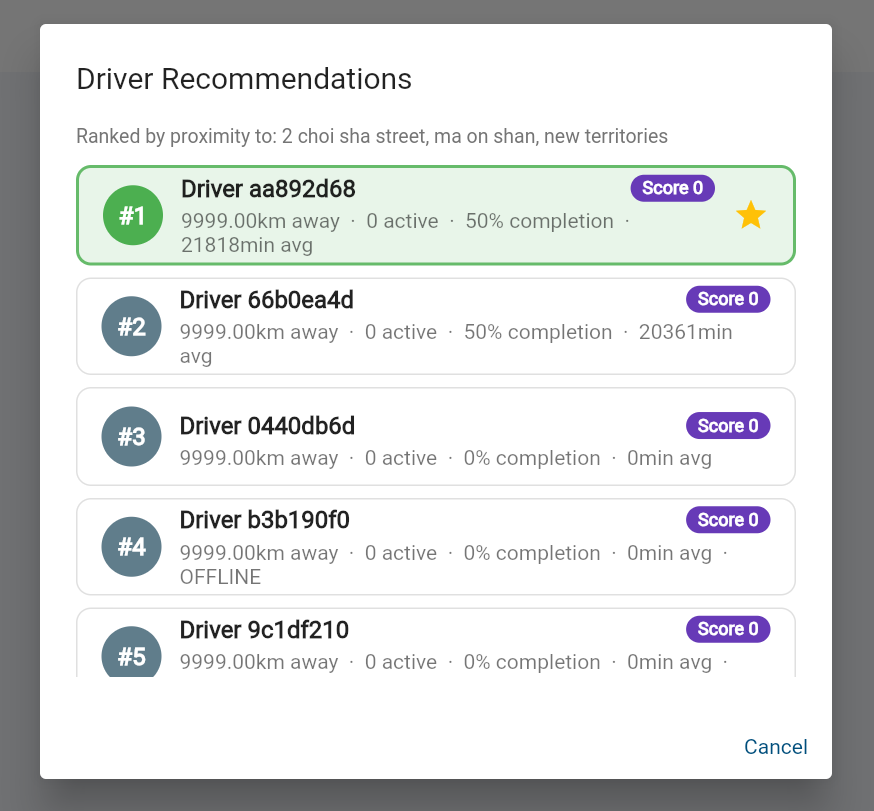
\includegraphics[width=0.7\textwidth]{ss-a7}
  \caption{Driver recommendation scores (A7).}
  \label{fig:ss-a7}
\end{figure}

\begin{figure}[H]
  \centering
  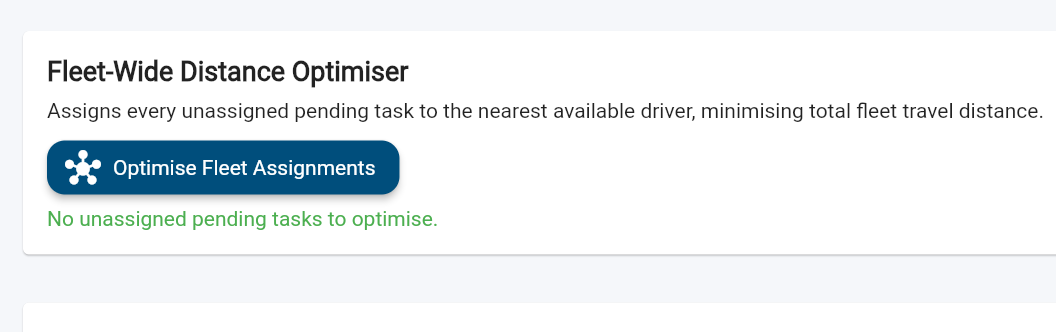
\includegraphics[width=0.7\textwidth]{ss-a8}
  \caption{Fleet-wide optimisation assignments (A8).}
  \label{fig:ss-a8}
\end{figure}

\begin{figure}[H]
  \centering
  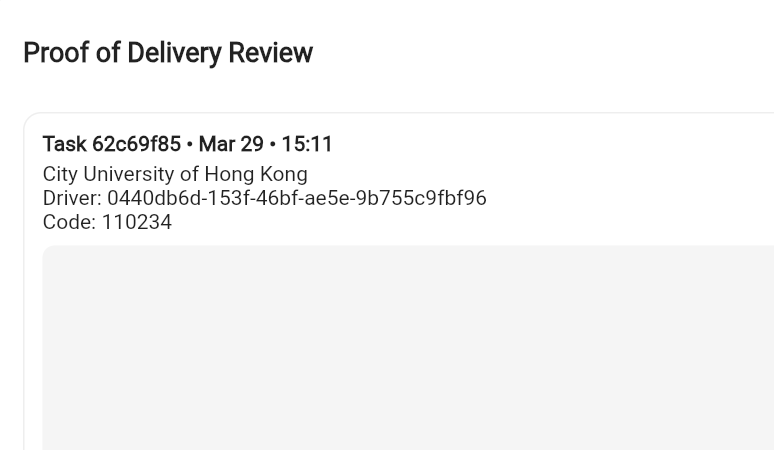
\includegraphics[width=0.7\textwidth]{ss-a9}
  \caption{Proof-of-delivery review panel (A9).}
  \label{fig:ss-a9}
\end{figure}

\begin{figure}[H]
  \centering
  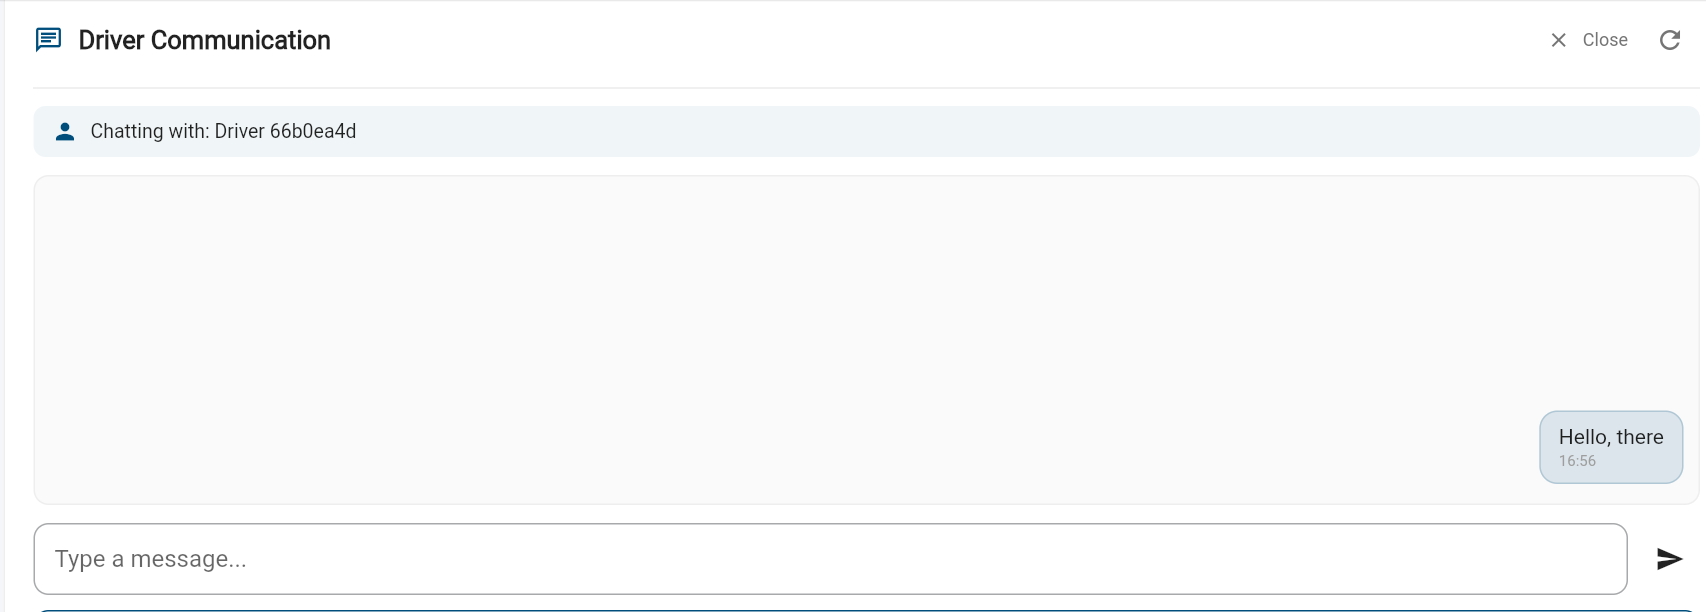
\includegraphics[width=0.7\textwidth]{ss-a10}
  \caption{Admin-to-driver chat message (A10).}
  \label{fig:ss-a10}
\end{figure}

\begin{figure}[H]
  \centering
  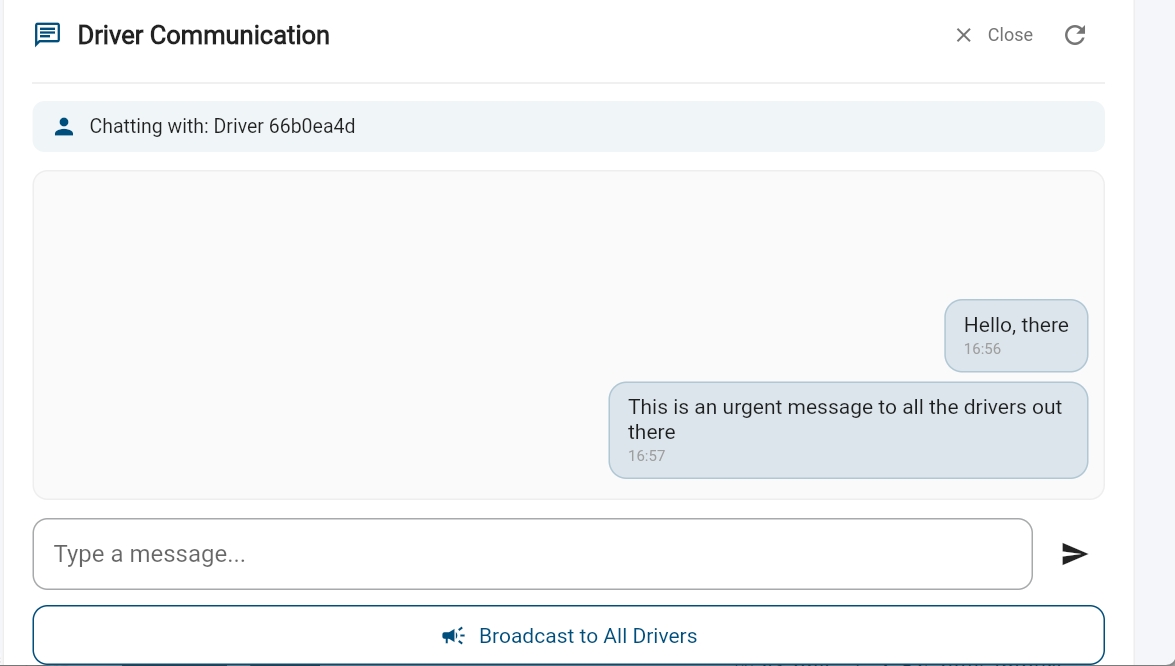
\includegraphics[width=0.7\textwidth]{ss-a11}
  \caption{Broadcast message to all drivers (A11).}
  \label{fig:ss-a11}
\end{figure}

\begin{figure}[H]
  \centering
  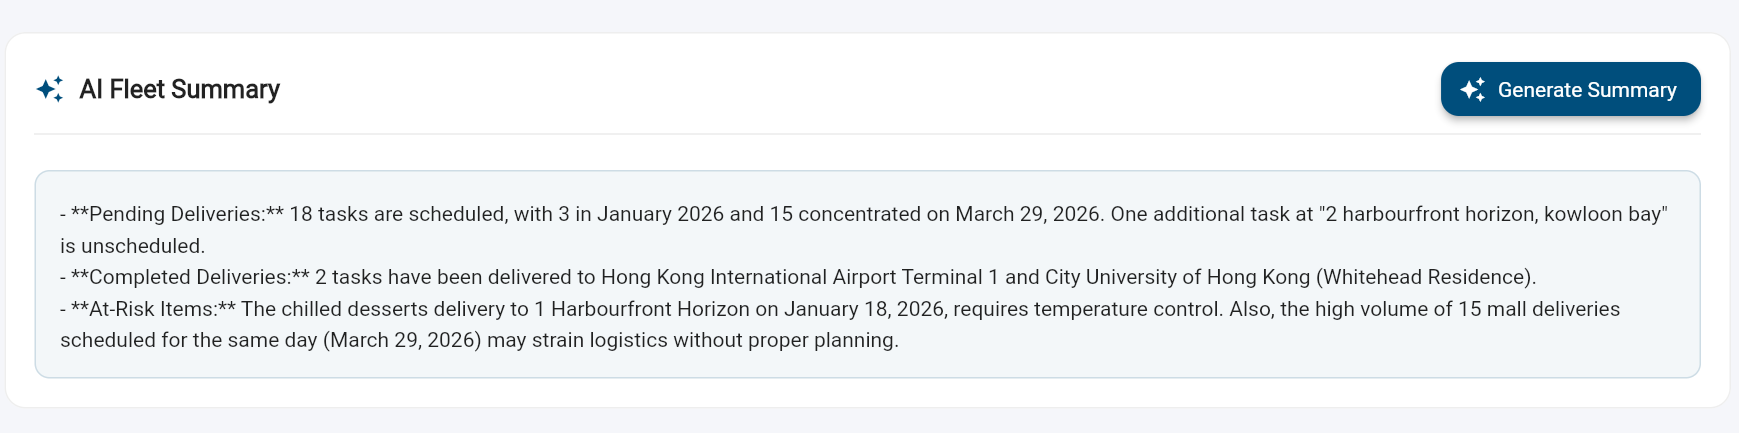
\includegraphics[width=0.7\textwidth]{ss-a12}
  \caption{AI-generated fleet summary (A12).}
  \label{fig:ss-a12}
\end{figure}

\clearpage
% ─────────────────────────────────────────────────────────────
\section{Functional Testing: Driver Application}
\label{sec:func-driver}

Table~\ref{tab:func-driver} lists the driver-side test cases executed on the
physical Samsung Galaxy~A54 device.

\begin{longtable}{c p{3.4cm} p{4.2cm} c c}
  \caption{Driver application functional test cases.}
  \label{tab:func-driver} \\
  \toprule
  \textbf{ID} & \textbf{Test Case} & \textbf{Expected Result} & \textbf{Pass} & \textbf{Fig.} \\
  \midrule
  \endfirsthead
  \toprule
  \textbf{ID} & \textbf{Test Case} & \textbf{Expected Result} & \textbf{Pass} & \textbf{Fig.} \\
  \midrule
  \endhead
  \midrule
  \multicolumn{5}{r}{\footnotesize\itshape Continued on next page} \\
  \endfoot
  \bottomrule
  \endlastfoot

  D1 & Login with driver credentials
     & Task list displayed with assigned deliveries
     & \checkmark
     & \ref{fig:ss-d1} \\

  D2 & View task details
     & Address, notes, priority, and time window shown
     & \checkmark
     & \ref{fig:ss-d2} \\

  D3 & Mark task as in-transit
     & Status badge updates to \emph{in-transit} in real-time
     & \checkmark
     & \ref{fig:ss-d3} \\

  D4 & Capture proof-of-delivery photo
     & Camera opens; photo uploaded to Supabase Storage; URL saved to task
     & \checkmark
     & \ref{fig:ss-d4} \\

  D5 & Mark task as delivered (with PoD)
     & Task moves to \emph{delivered}; PoD photo visible in admin review
     & \checkmark
     & \ref{fig:ss-d5} \\

  D6 & AI task summary
     & Natural-language summary of remaining tasks displayed
     & \checkmark
     & \ref{fig:ss-d6} \\

  D7 & AI chat (free-form question)
     & Contextual response returned within 3 seconds
     & \checkmark
     & \ref{fig:ss-d7} \\

  D8 & Agentic AI suggestion
     & Structured suggestion with one-tap action chip displayed
     & \checkmark
     & \ref{fig:ss-d8} \\

  D9 & Execute agentic action (confirm)
     & Action executed (e.g.\ task status changed); confirmation shown
     & \checkmark
     & \ref{fig:ss-d9} \\

  D10 & Mid-shift re-sequencing
      & Task order updates based on current GPS; resequence banner shown
      & \checkmark
      & \ref{fig:ss-d10} \\

  D11 & Offline delivery completion
      & Task marked delivered locally; sync icon appears; uploads on reconnect
      & \checkmark
      & \ref{fig:ss-d11} \\

  D12 & Receive chat message from admin
      & Message appears in chat tab; notification badge shown
      & \checkmark
      & \ref{fig:ss-d12} \\

  D13 & Toggle availability status
      & Status updates to available/offline; admin sees change in real-time
      & \checkmark
      & \ref{fig:ss-d13} \\

  D14 & Sign out
      & Session ended; login screen shown
      & \checkmark
      & \ref{fig:ss-d14} \\

  D15 & Scan barcode to locate task
      & Camera opens; scanned code matches task; task highlighted in list
      & \checkmark
      & --- \\
\end{longtable}

% ── Screenshot placeholders — Driver ──

\begin{figure}[H]
  \centering
  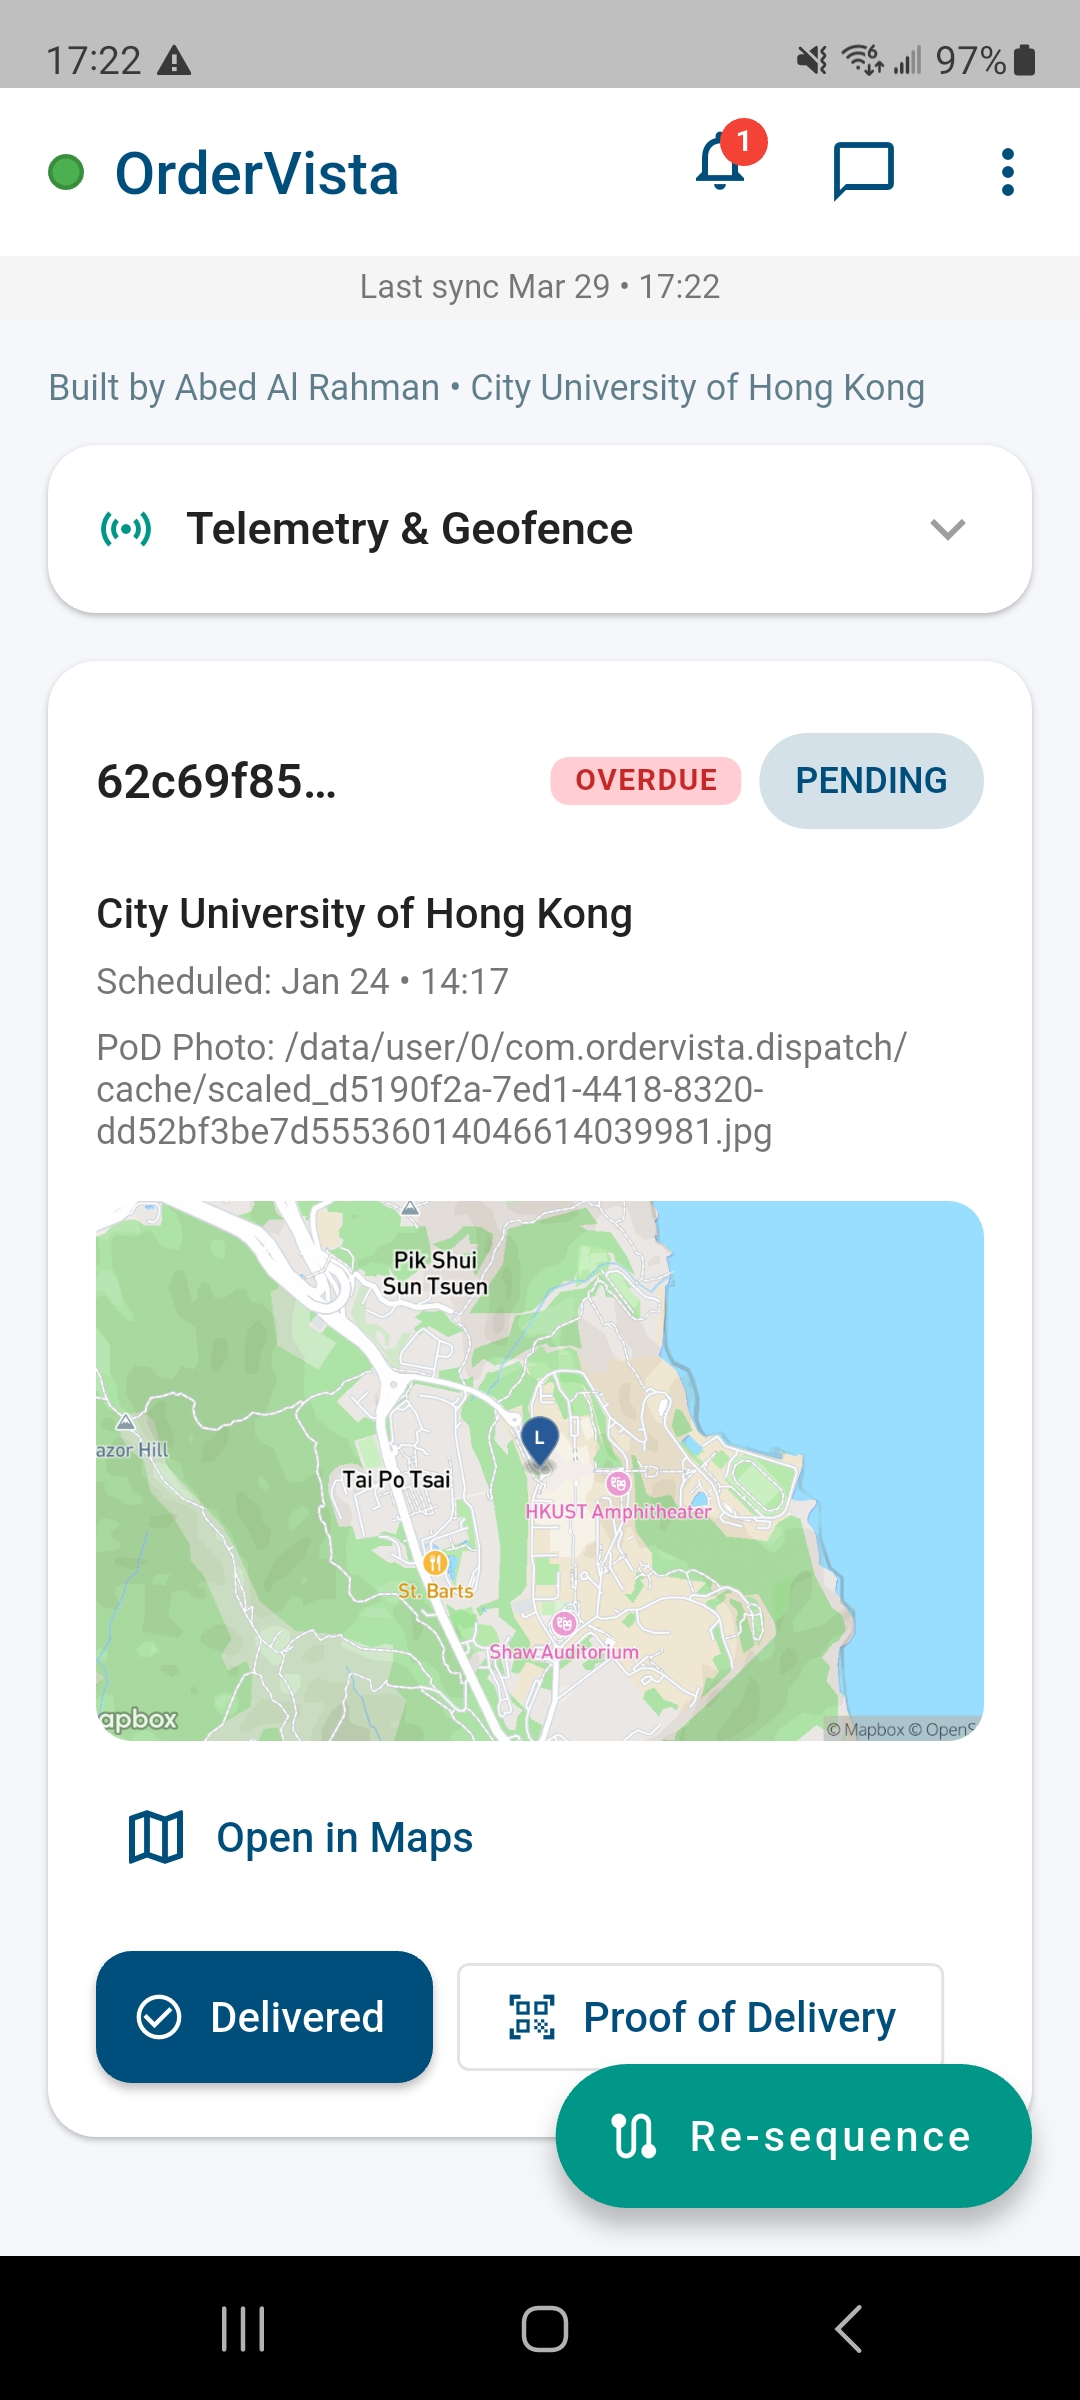
\includegraphics[width=0.45\textwidth]{ss-d1}
  \caption{Driver login screen (D1).}
  \label{fig:ss-d1}
\end{figure}

\begin{figure}[H]
  \centering
  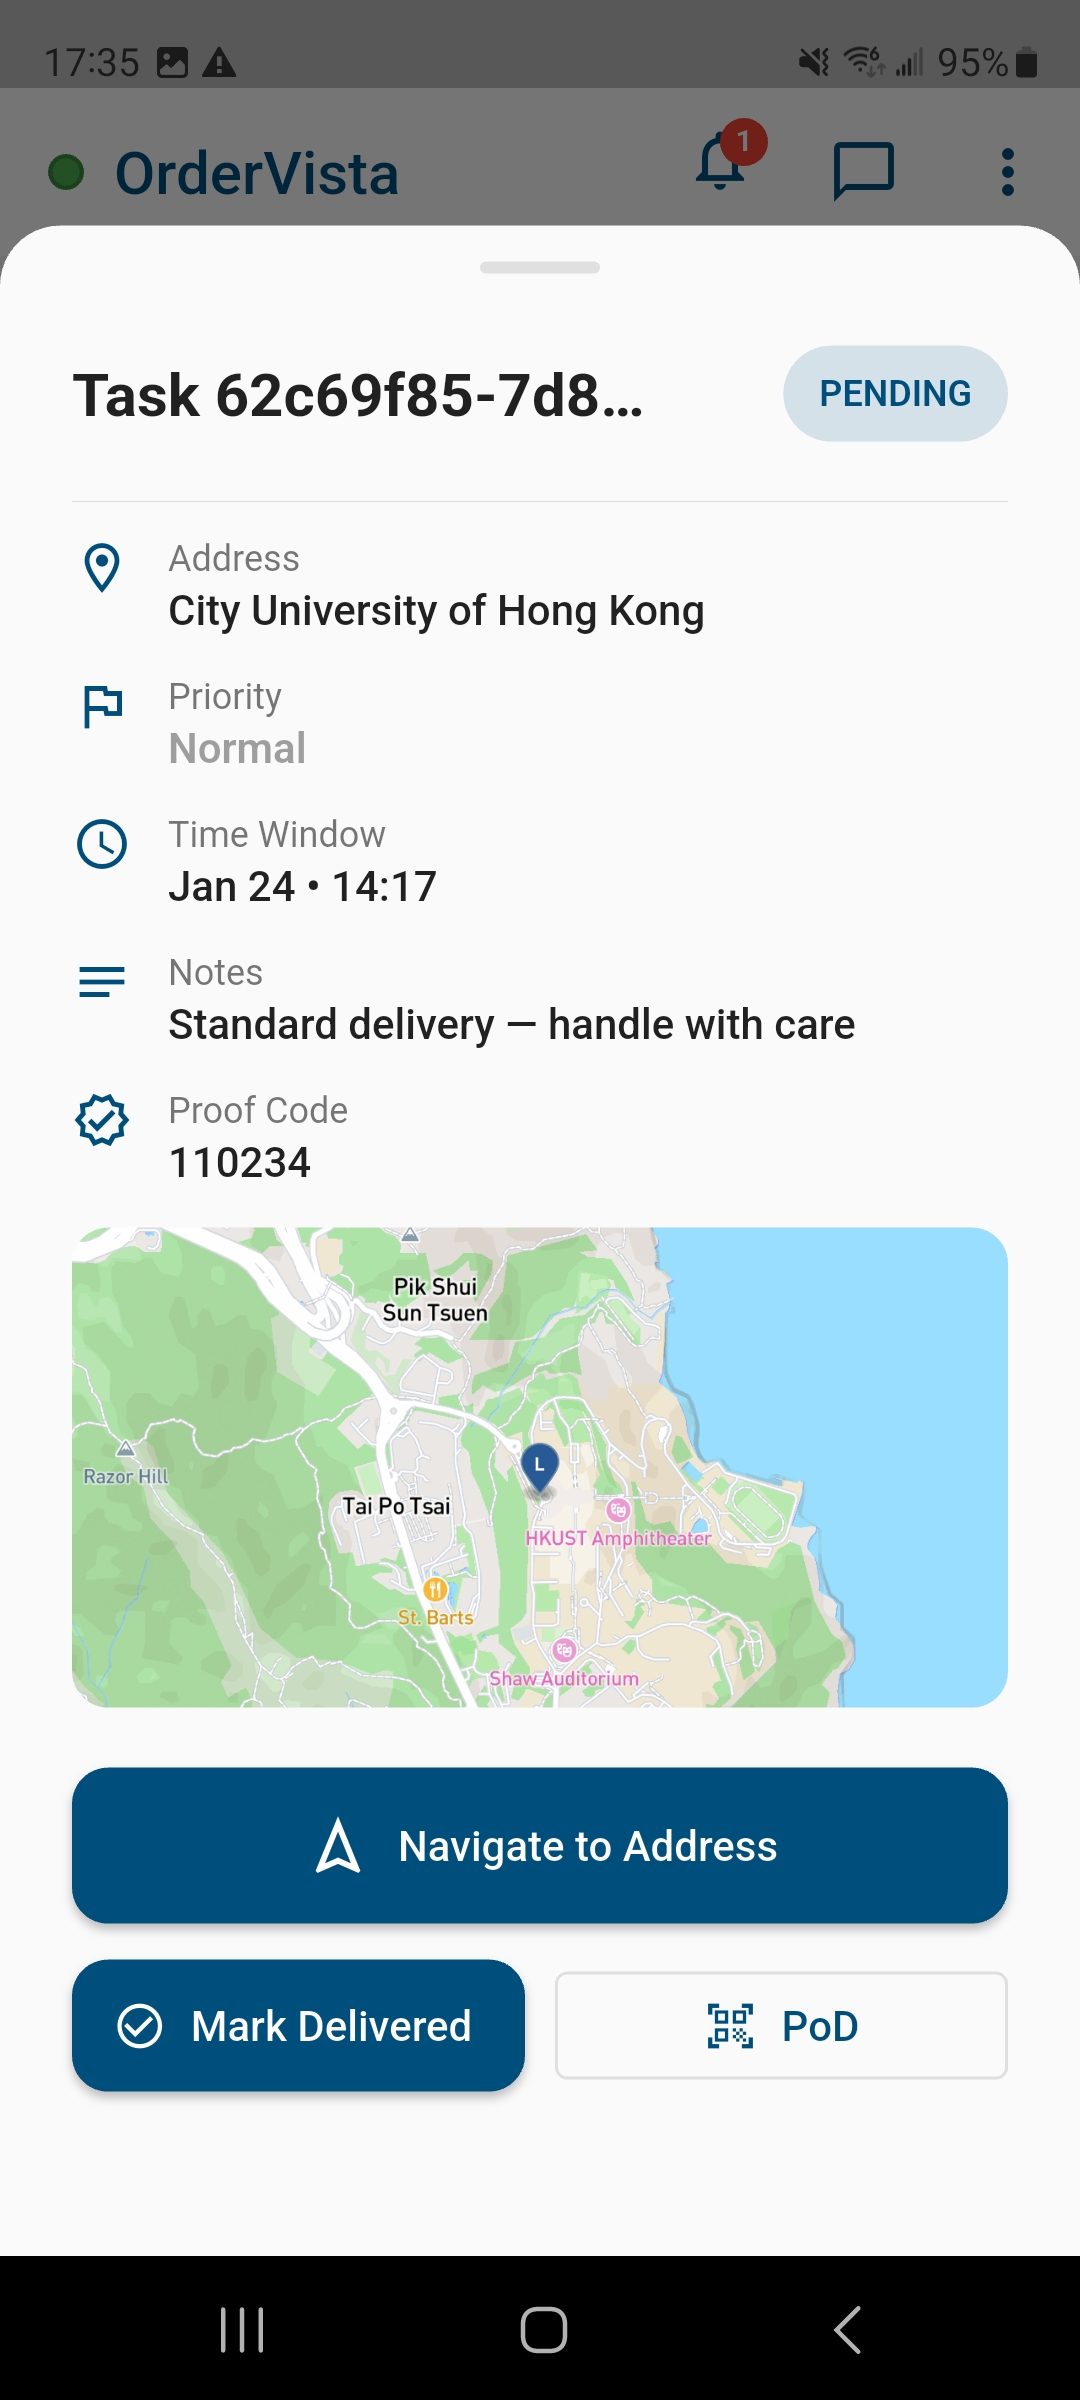
\includegraphics[width=0.45\textwidth]{ss-d2}
  \caption{Task detail view with address and time window (D2).}
  \label{fig:ss-d2}
\end{figure}

\begin{figure}[H]
  \centering
  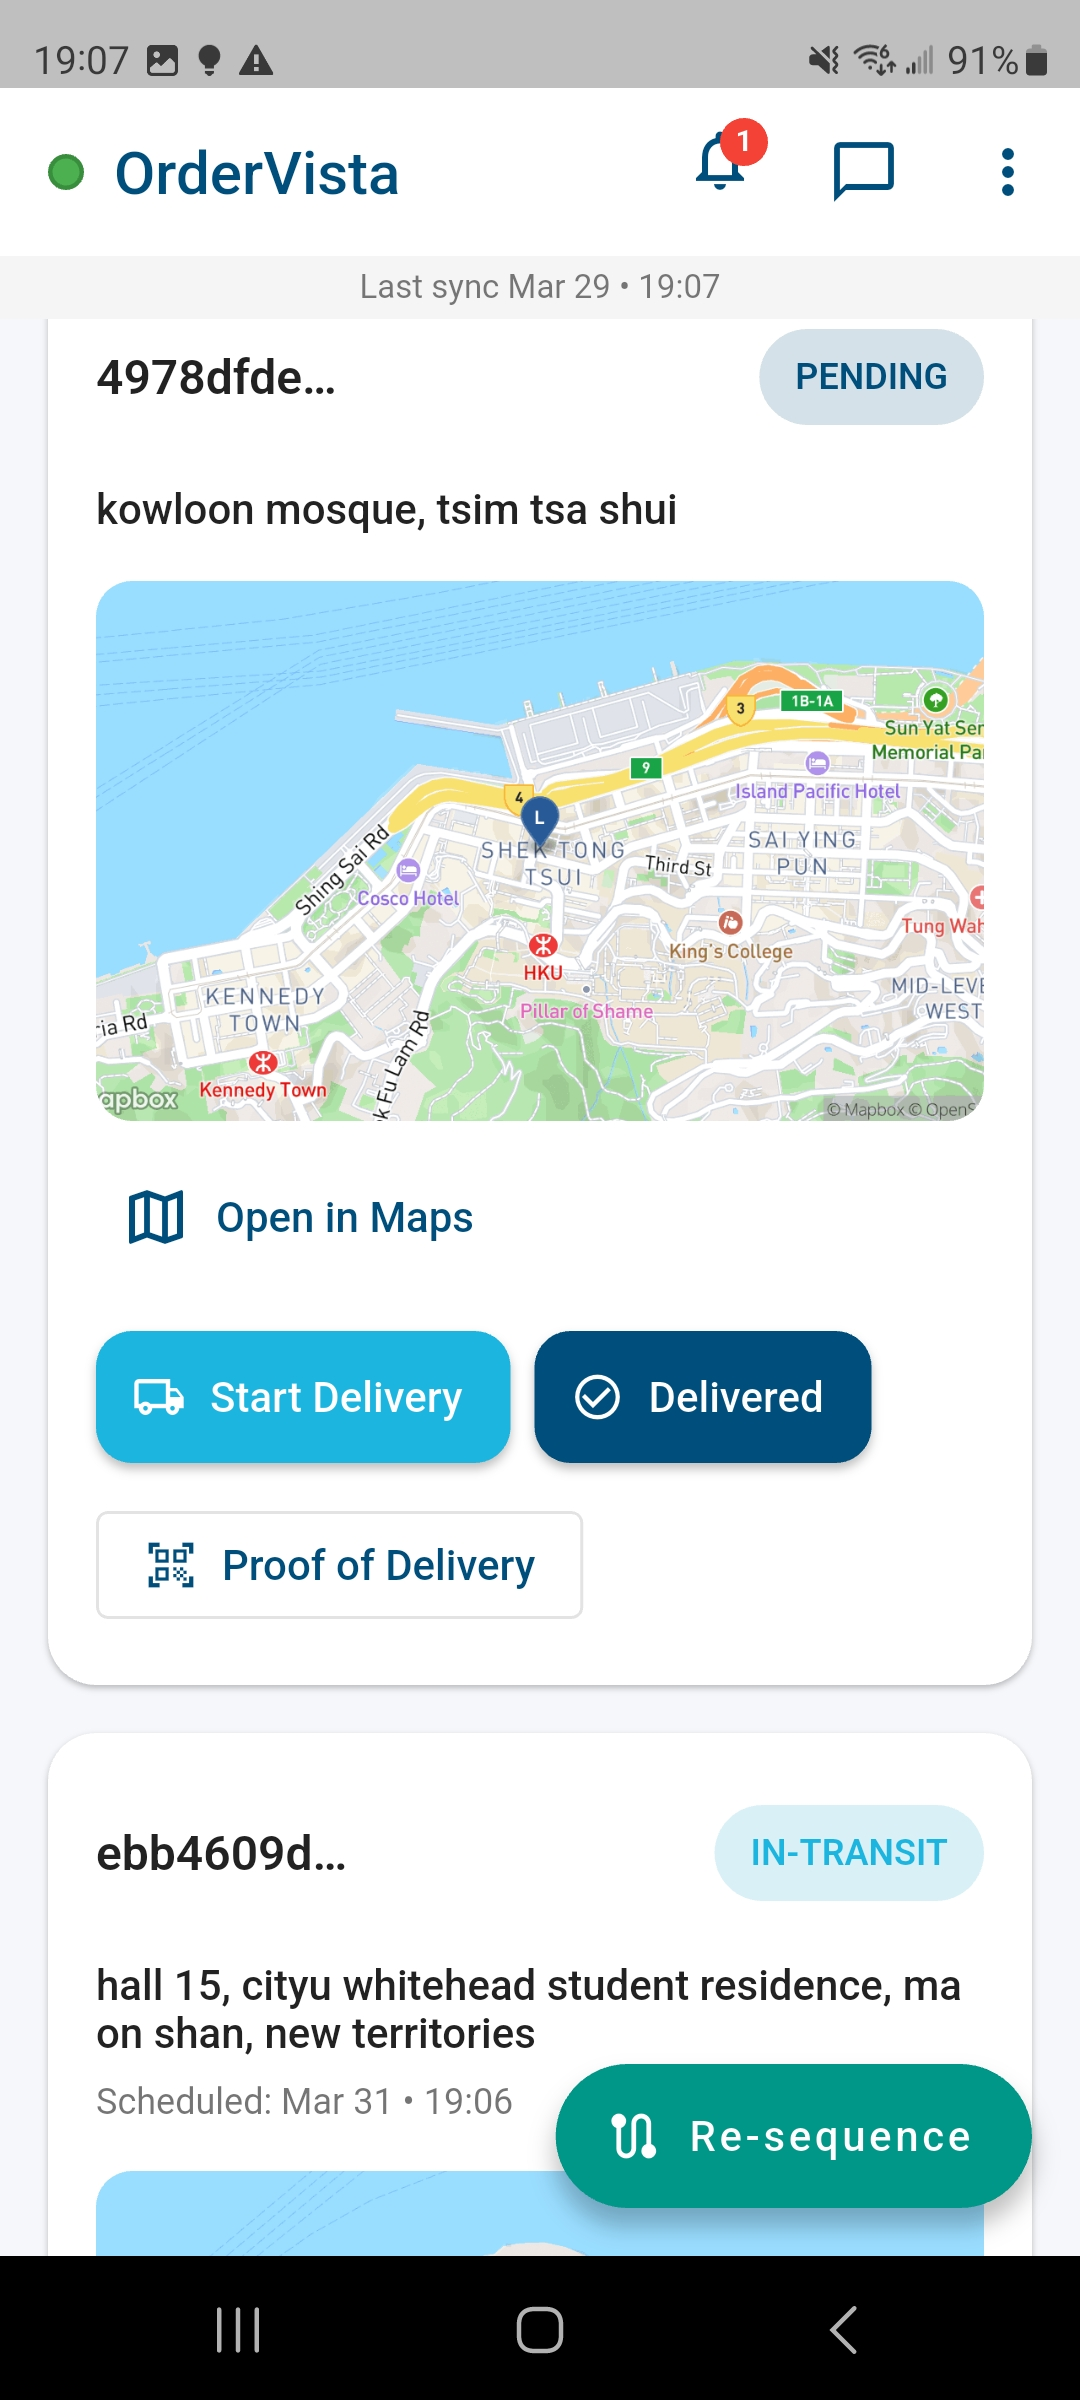
\includegraphics[width=0.45\textwidth]{ss-d3}
  \caption{Task marked as in-transit (D3).}
  \label{fig:ss-d3}
\end{figure}

\begin{figure}[H]
  \centering
  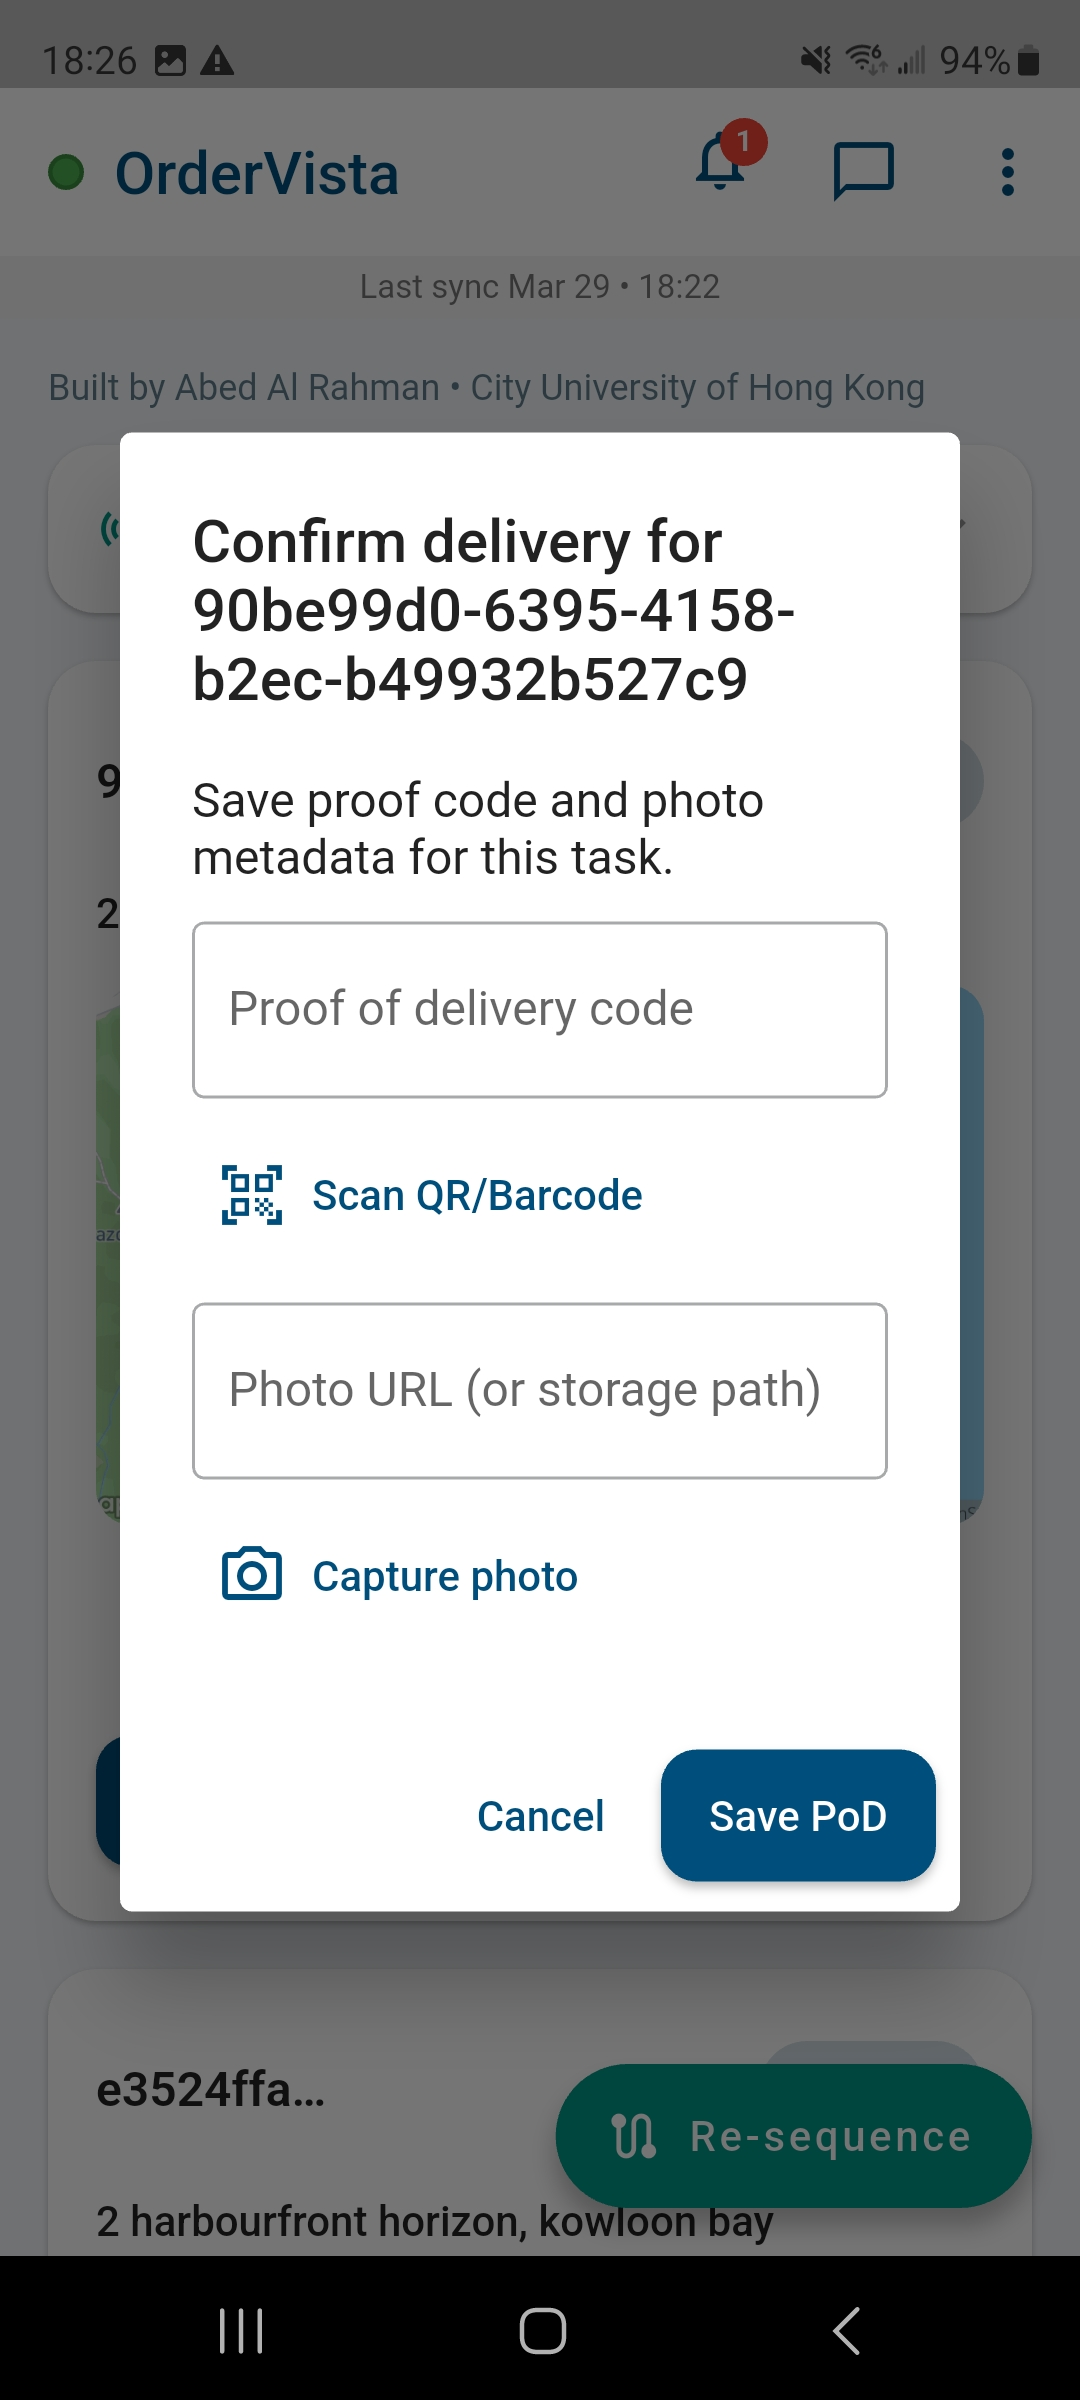
\includegraphics[width=0.45\textwidth]{ss-d4}
  \caption{Proof-of-delivery photo capture (D4).}
  \label{fig:ss-d4}
\end{figure}

\begin{figure}[H]
  \centering
  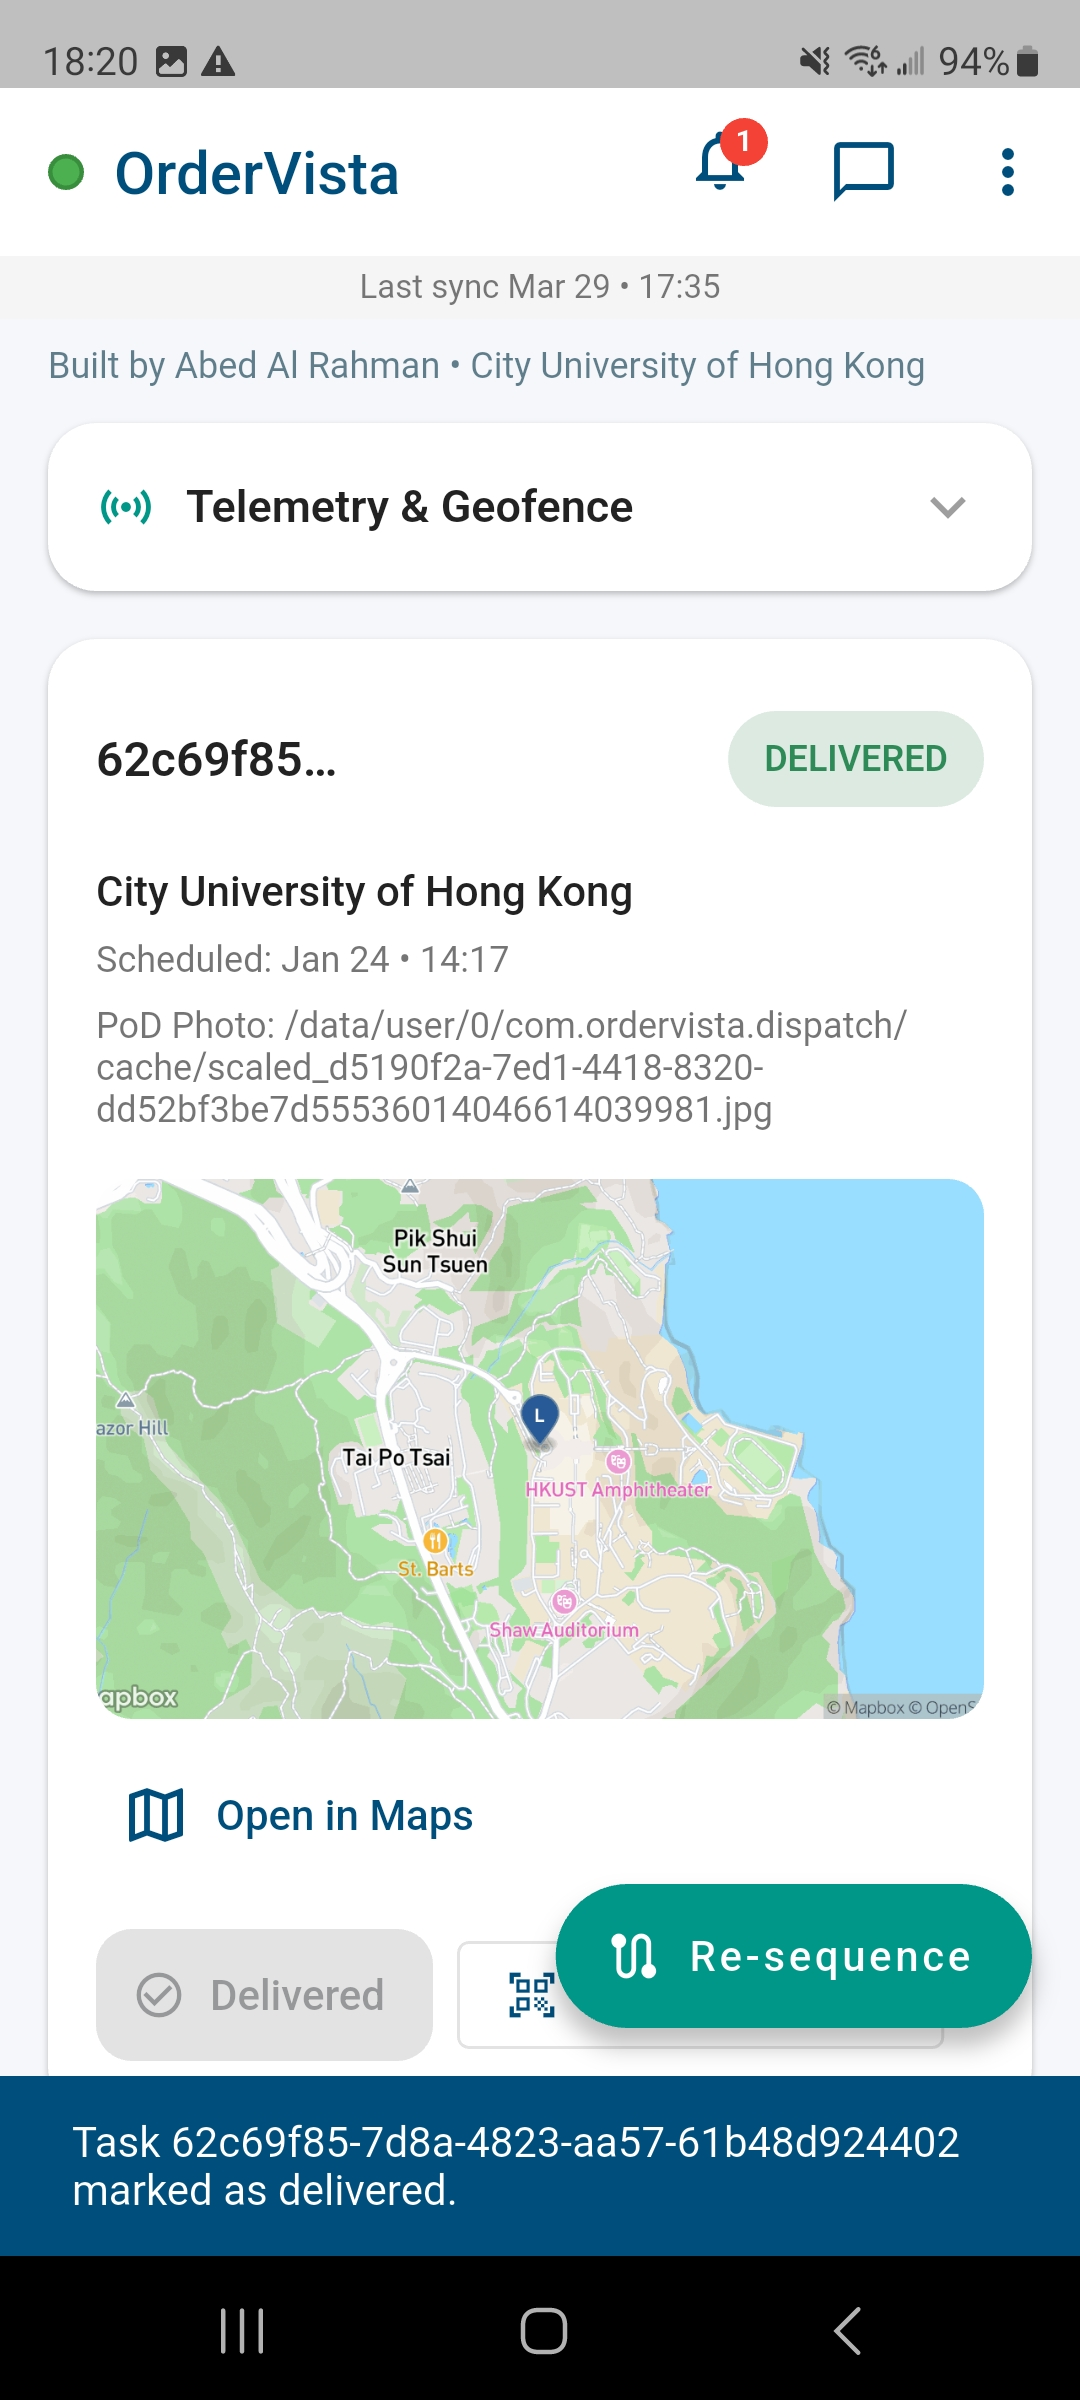
\includegraphics[width=0.45\textwidth]{ss-d5}
  \caption{Task marked as delivered with PoD confirmation (D5).}
  \label{fig:ss-d5}
\end{figure}

\begin{figure}[H]
  \centering
  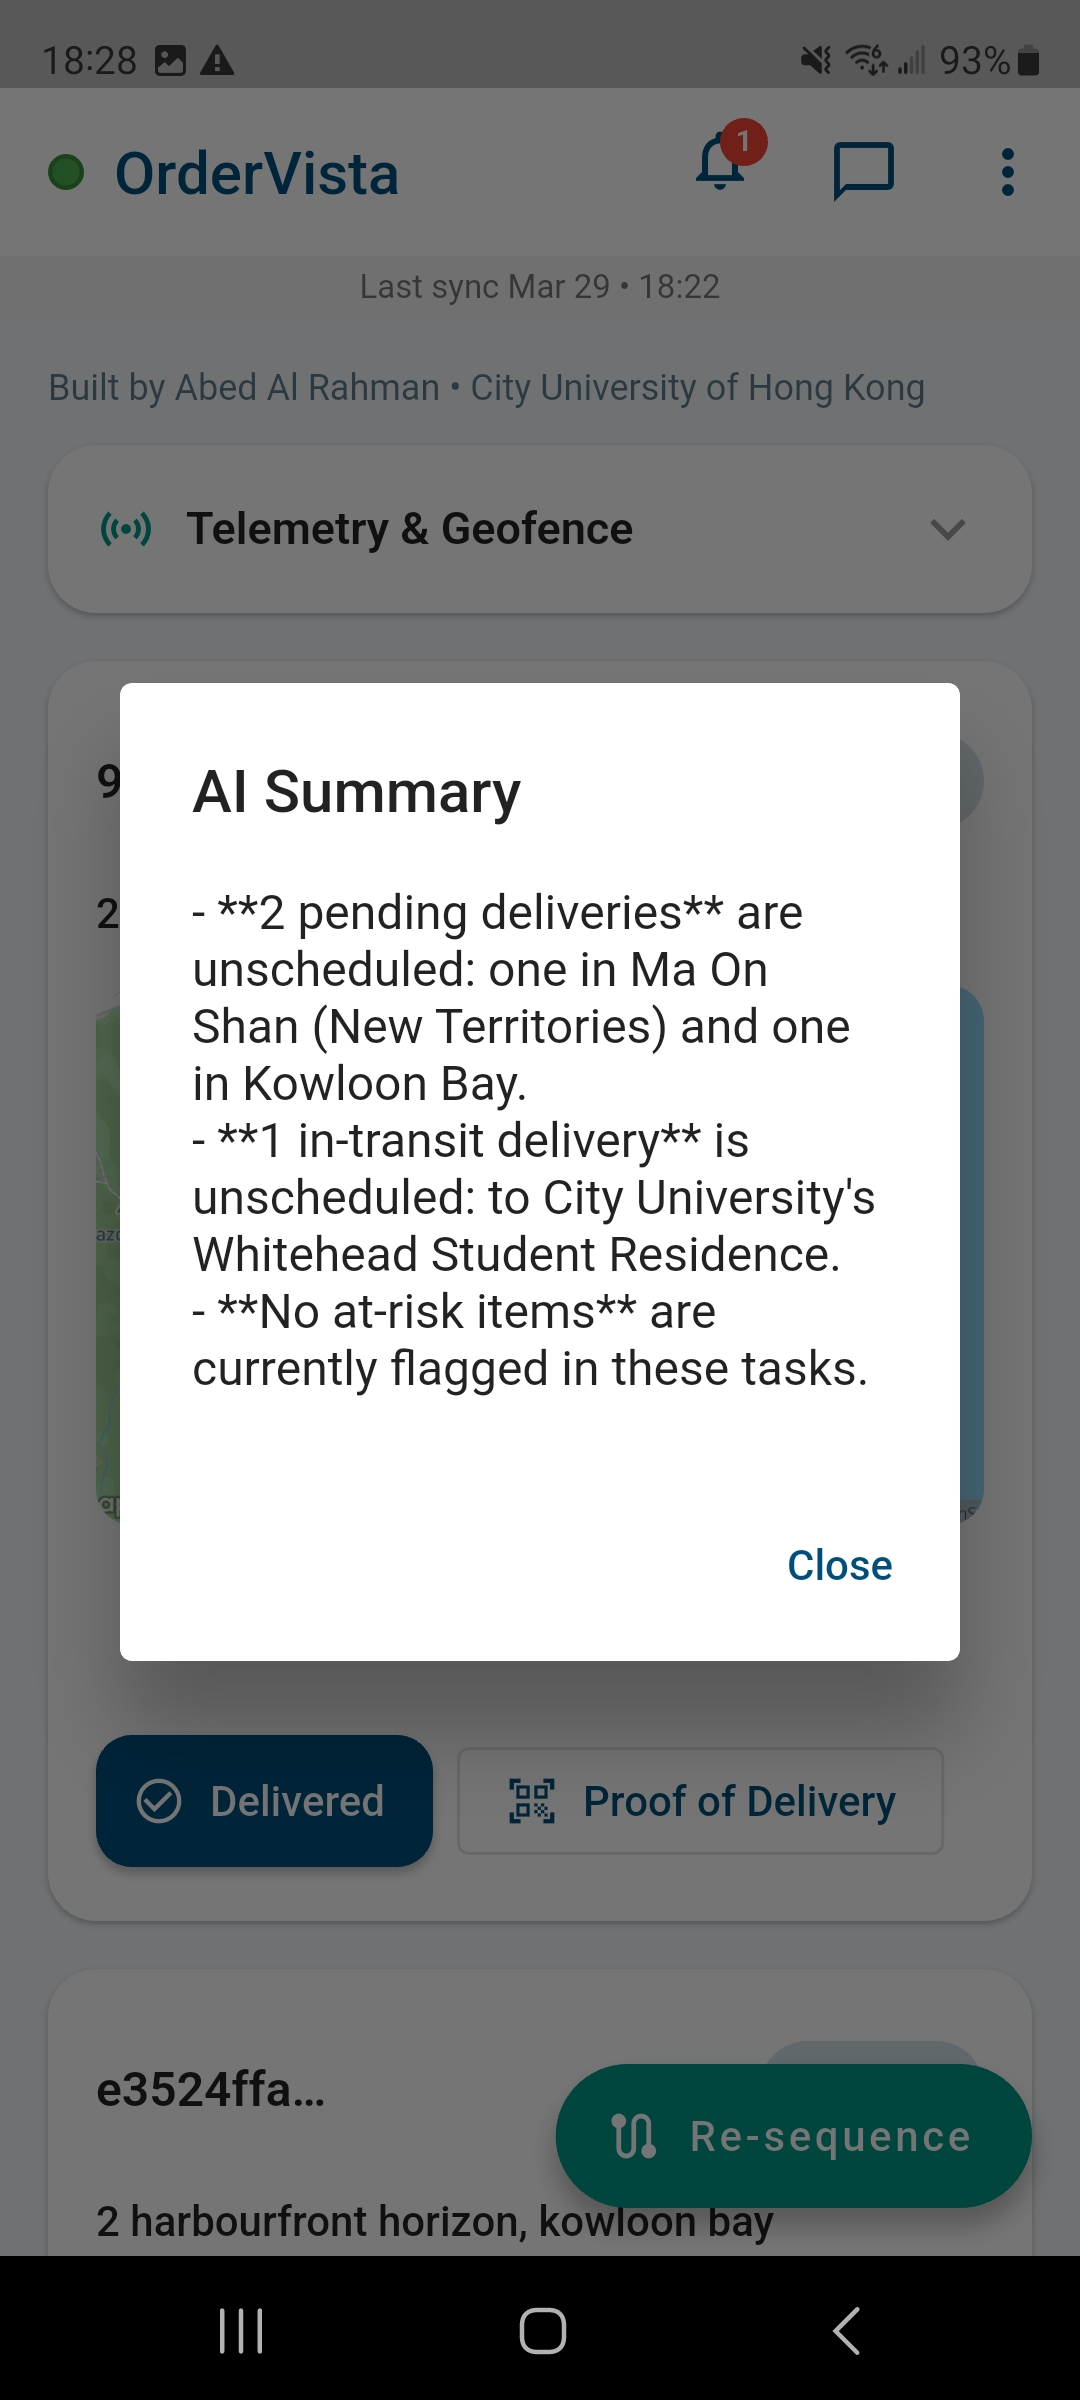
\includegraphics[width=0.45\textwidth]{ss-d6}
  \caption{AI task summary on driver device (D6).}
  \label{fig:ss-d6}
\end{figure}

\begin{figure}[H]
  \centering
  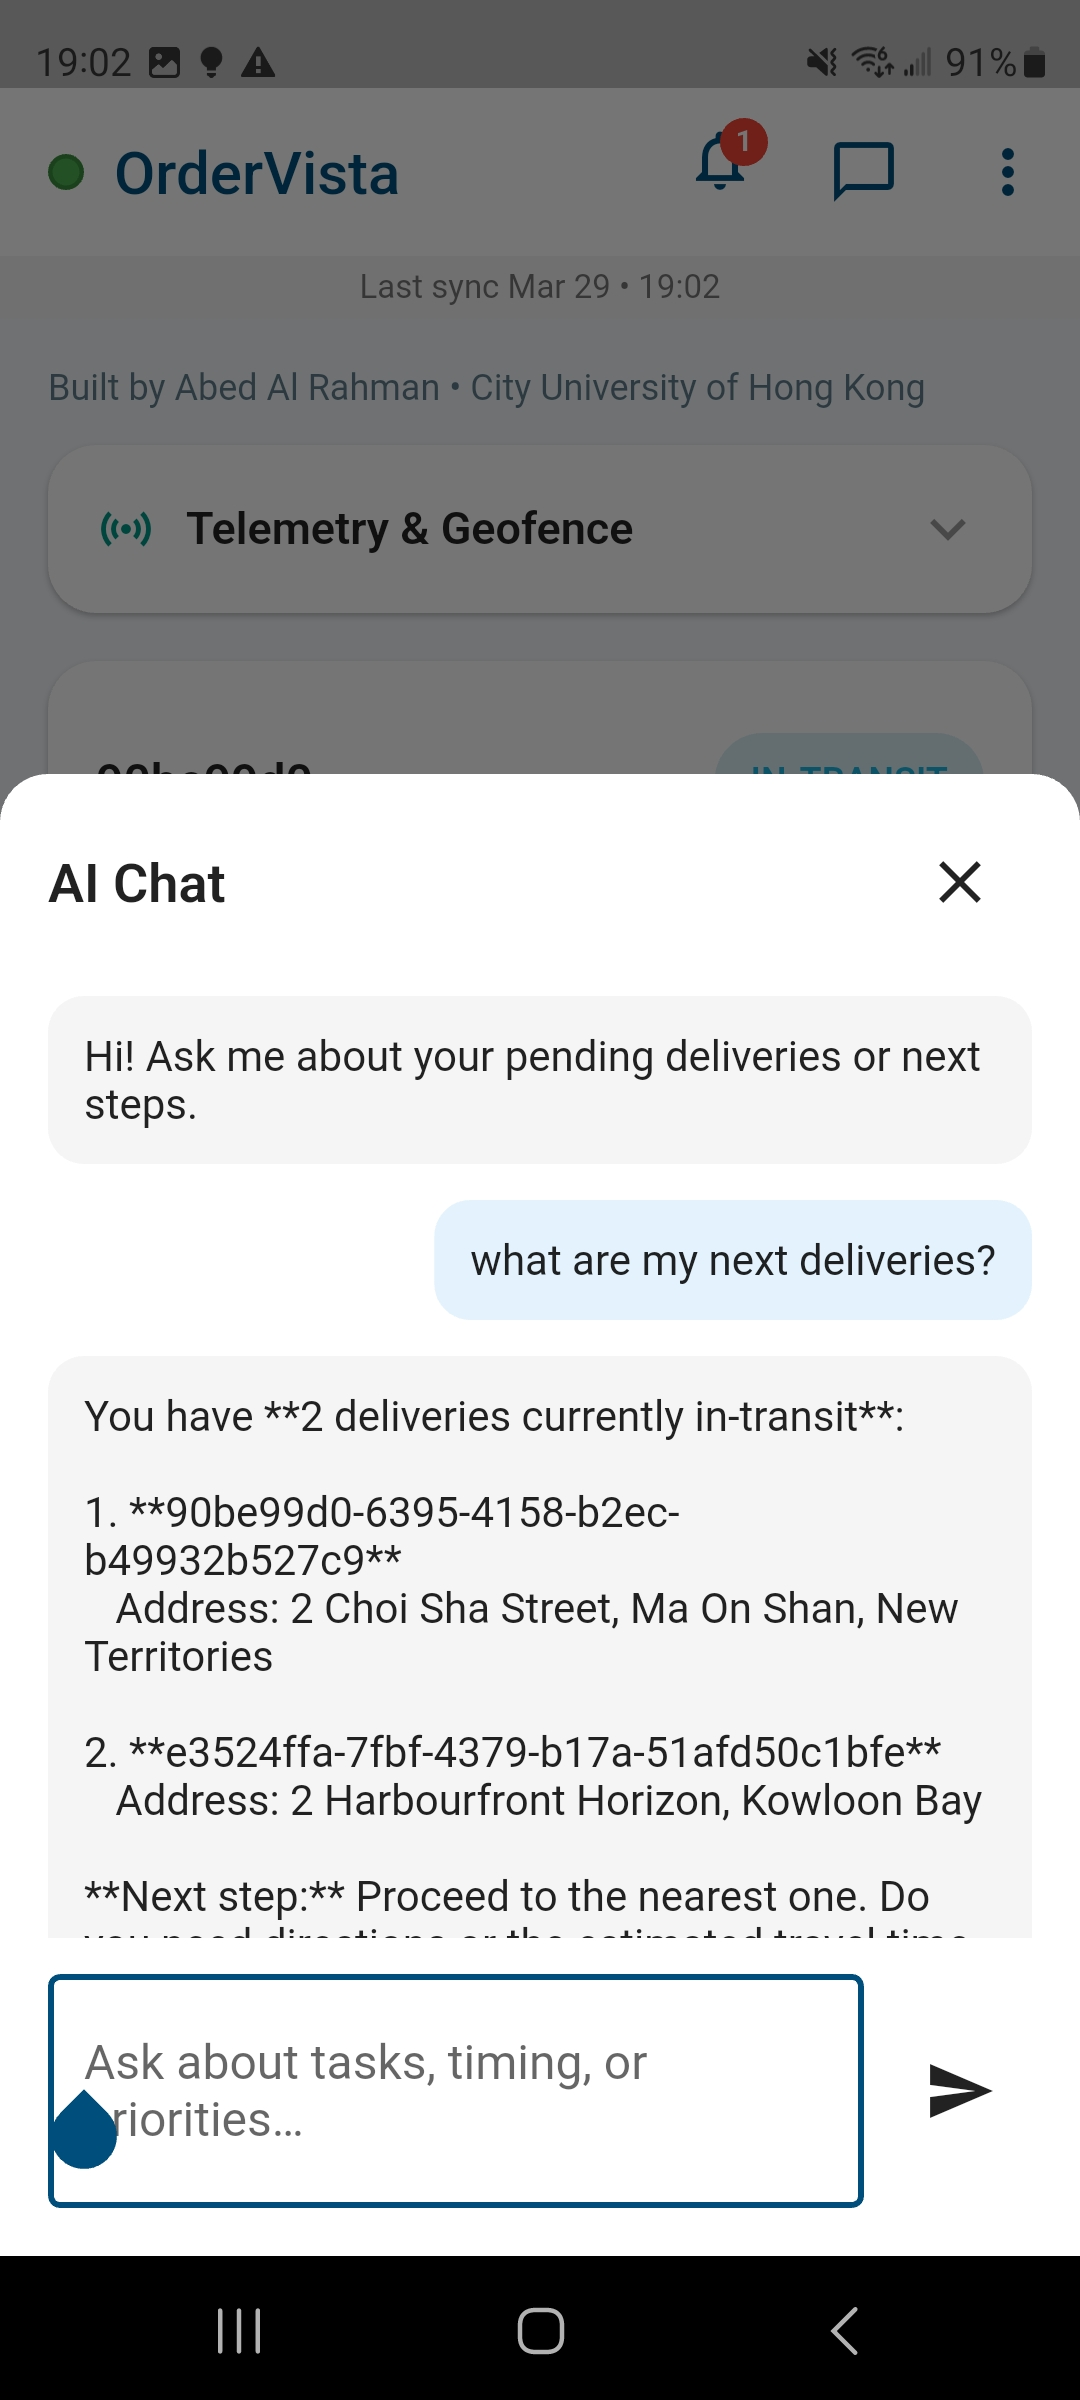
\includegraphics[width=0.45\textwidth]{ss-d7}
  \caption{AI free-form chat conversation (D7).}
  \label{fig:ss-d7}
\end{figure}

\begin{figure}[H]
  \centering
  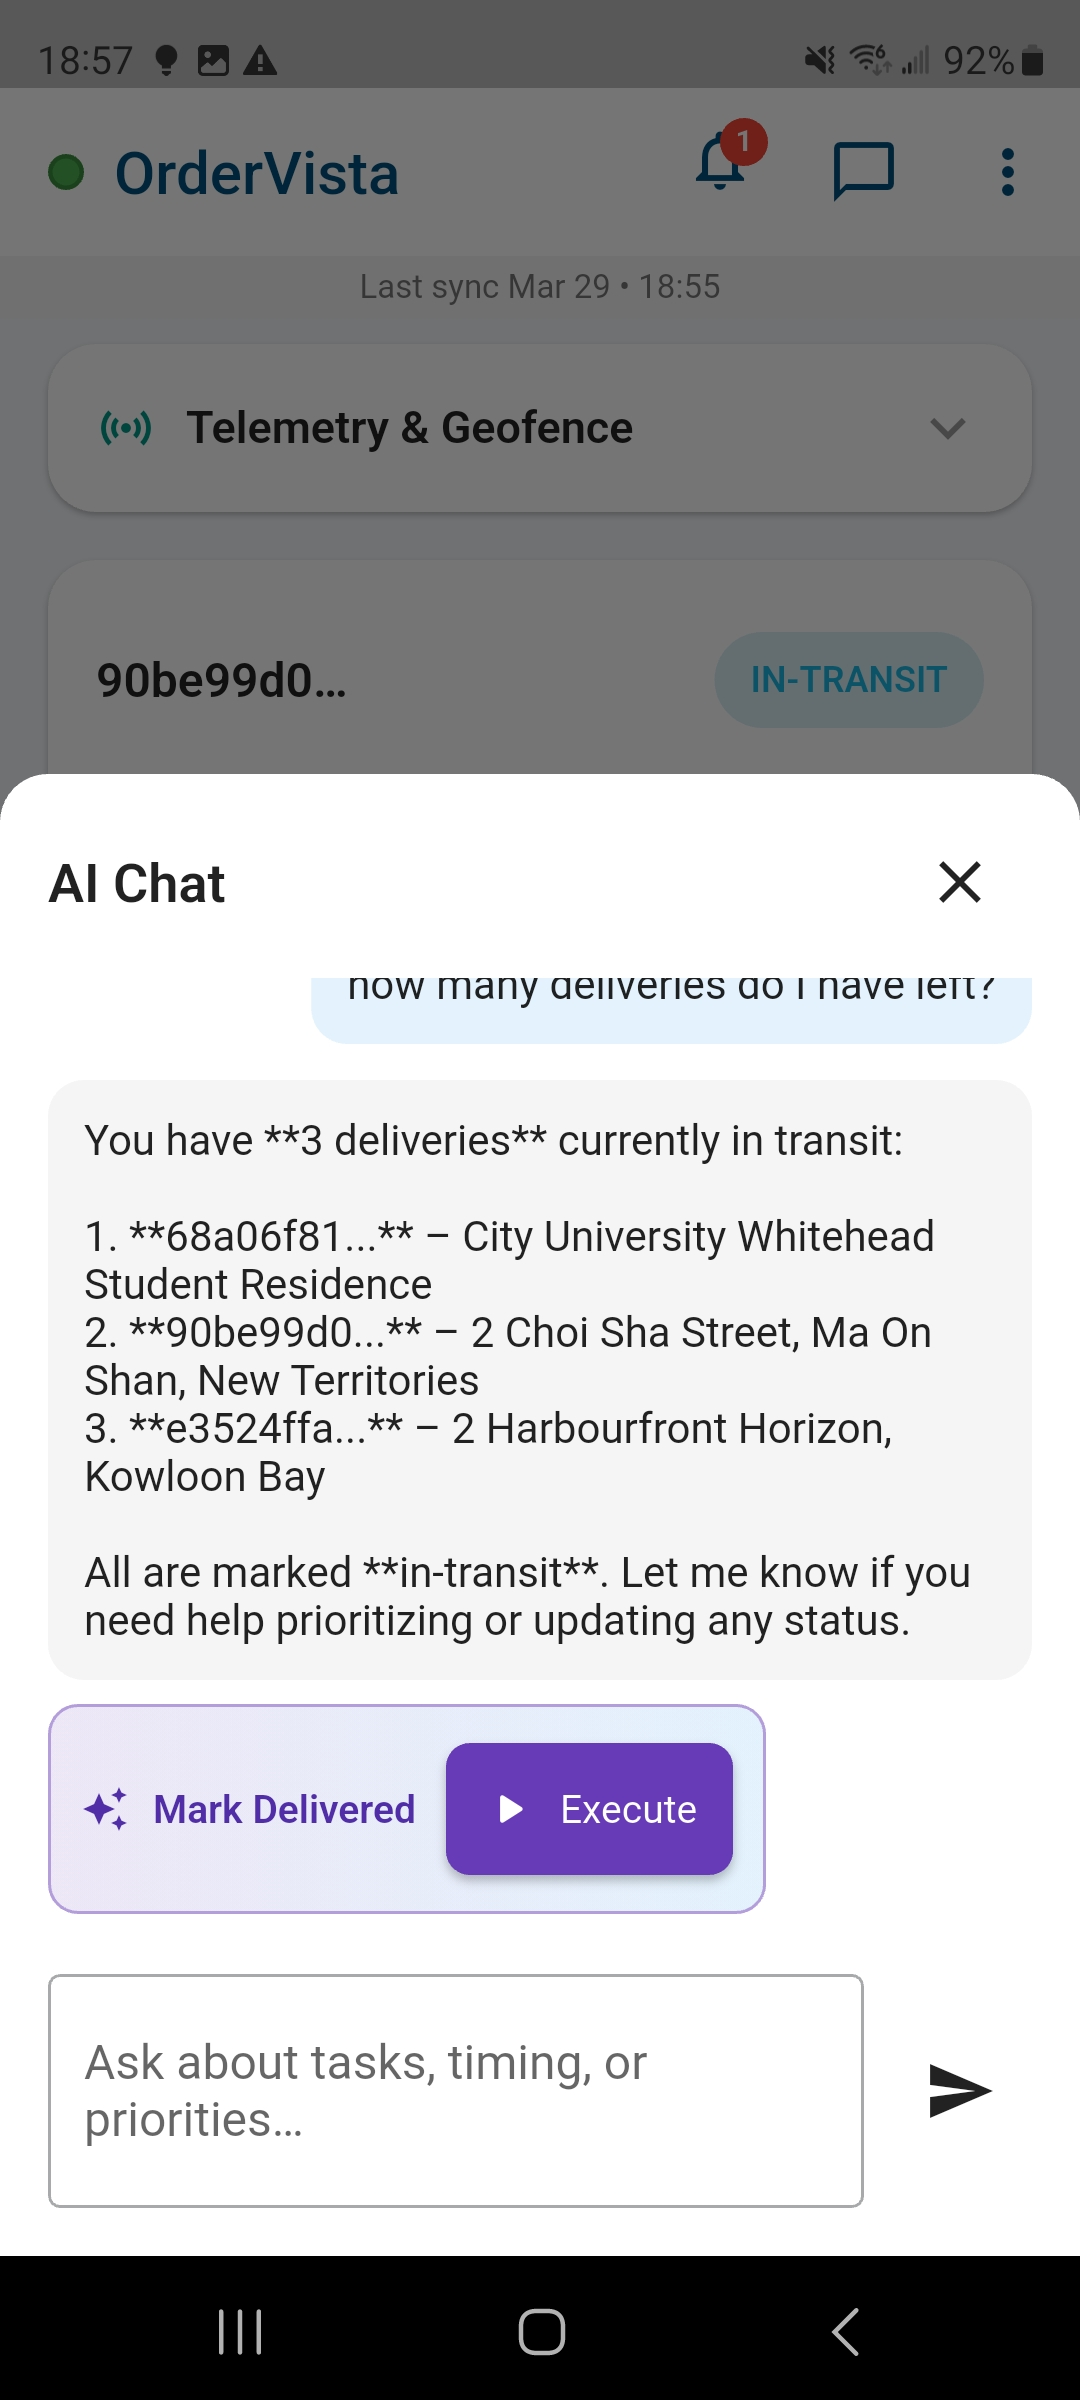
\includegraphics[width=0.45\textwidth]{ss-d8}
  \caption{Agentic AI suggestion with action chip (D8).}
  \label{fig:ss-d8}
\end{figure}

\begin{figure}[H]
  \centering
  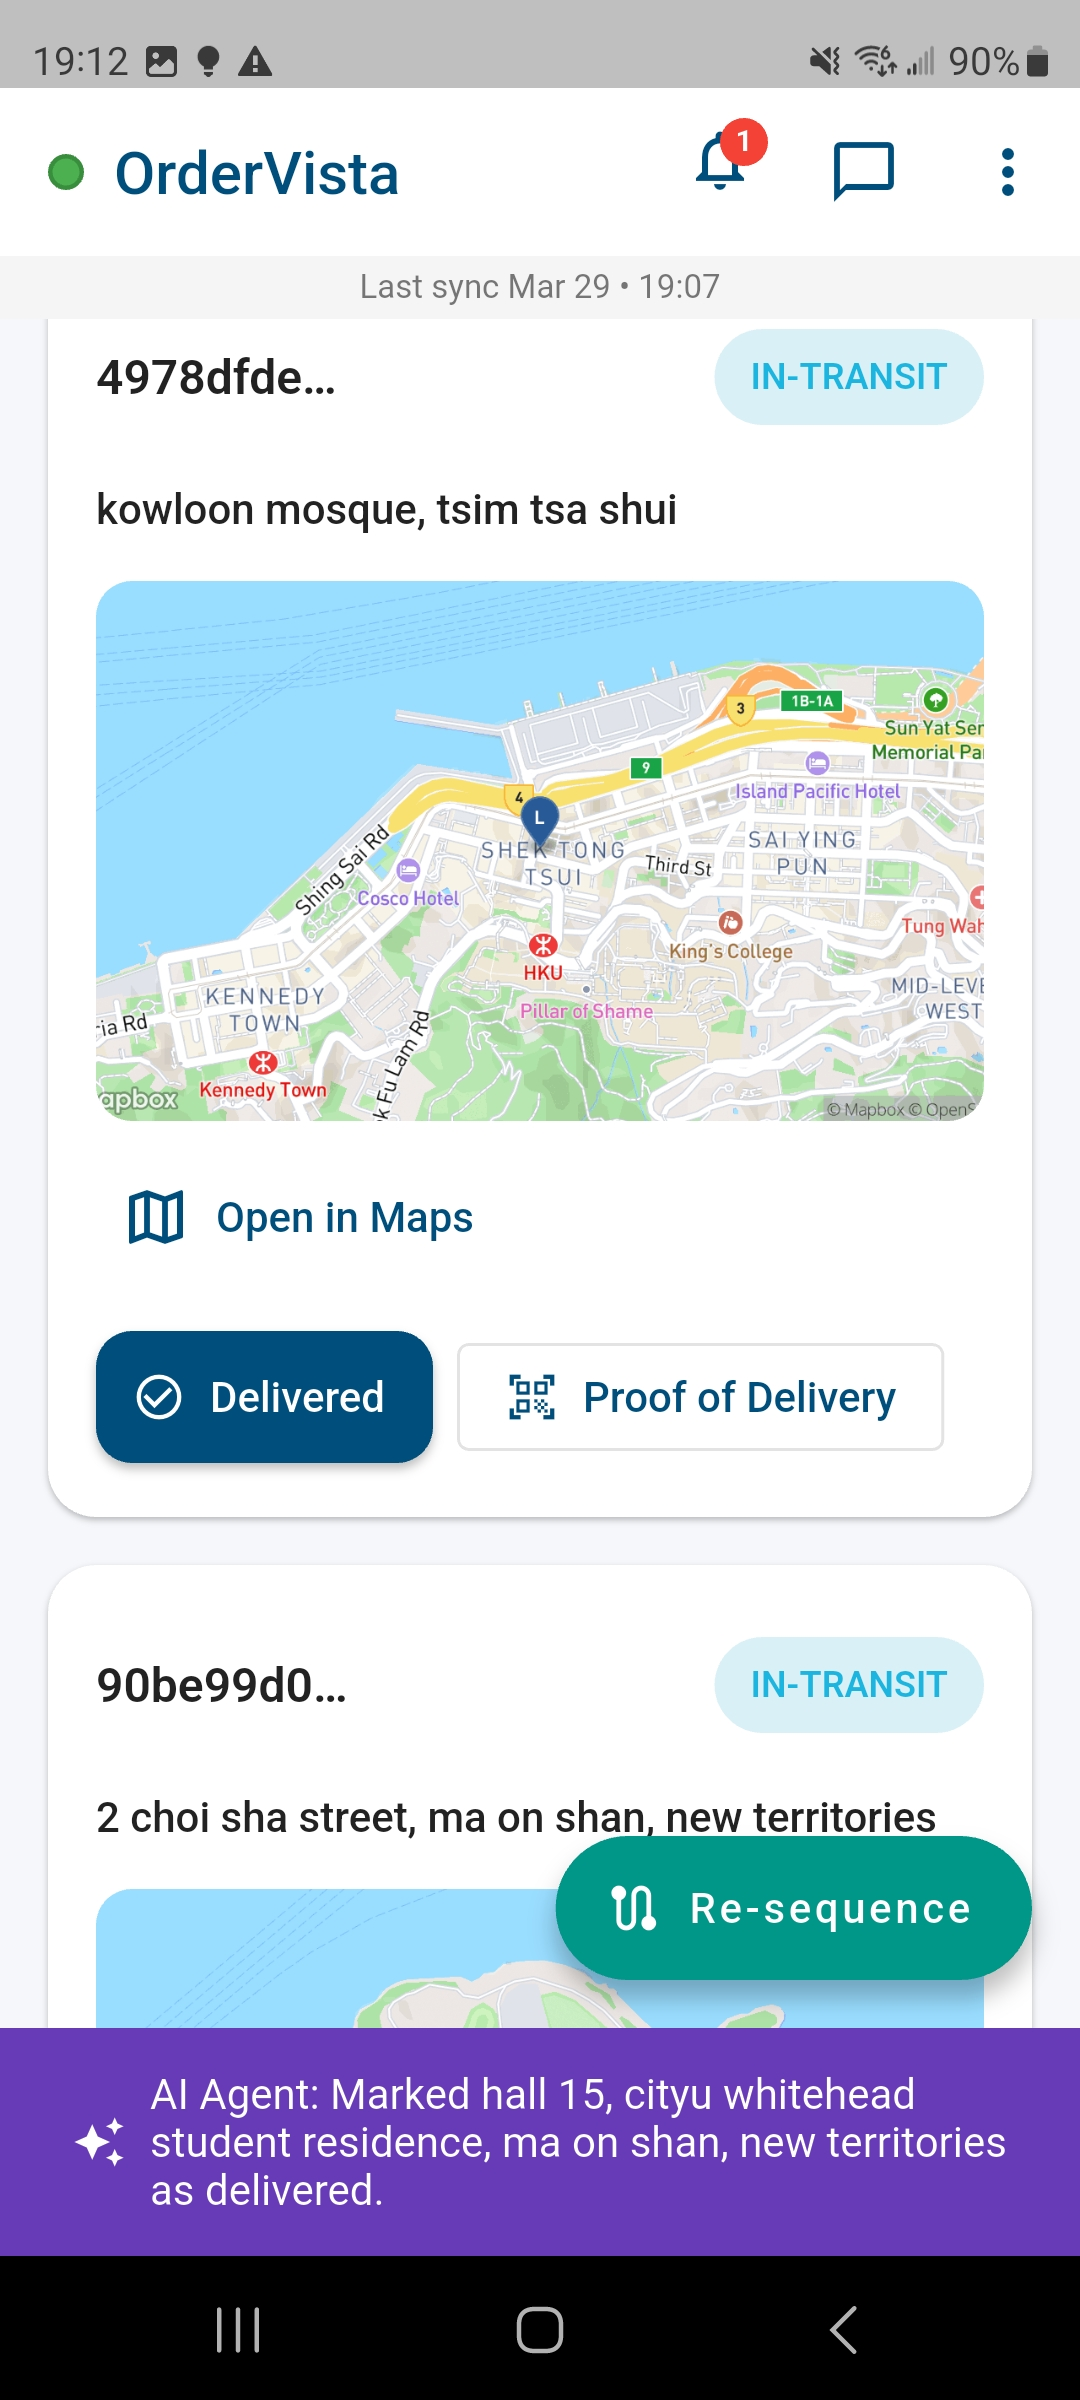
\includegraphics[width=0.45\textwidth]{ss-d9}
  \caption{Agentic action executed after user confirmation (D9).}
  \label{fig:ss-d9}
\end{figure}

\begin{figure}[H]
  \centering
  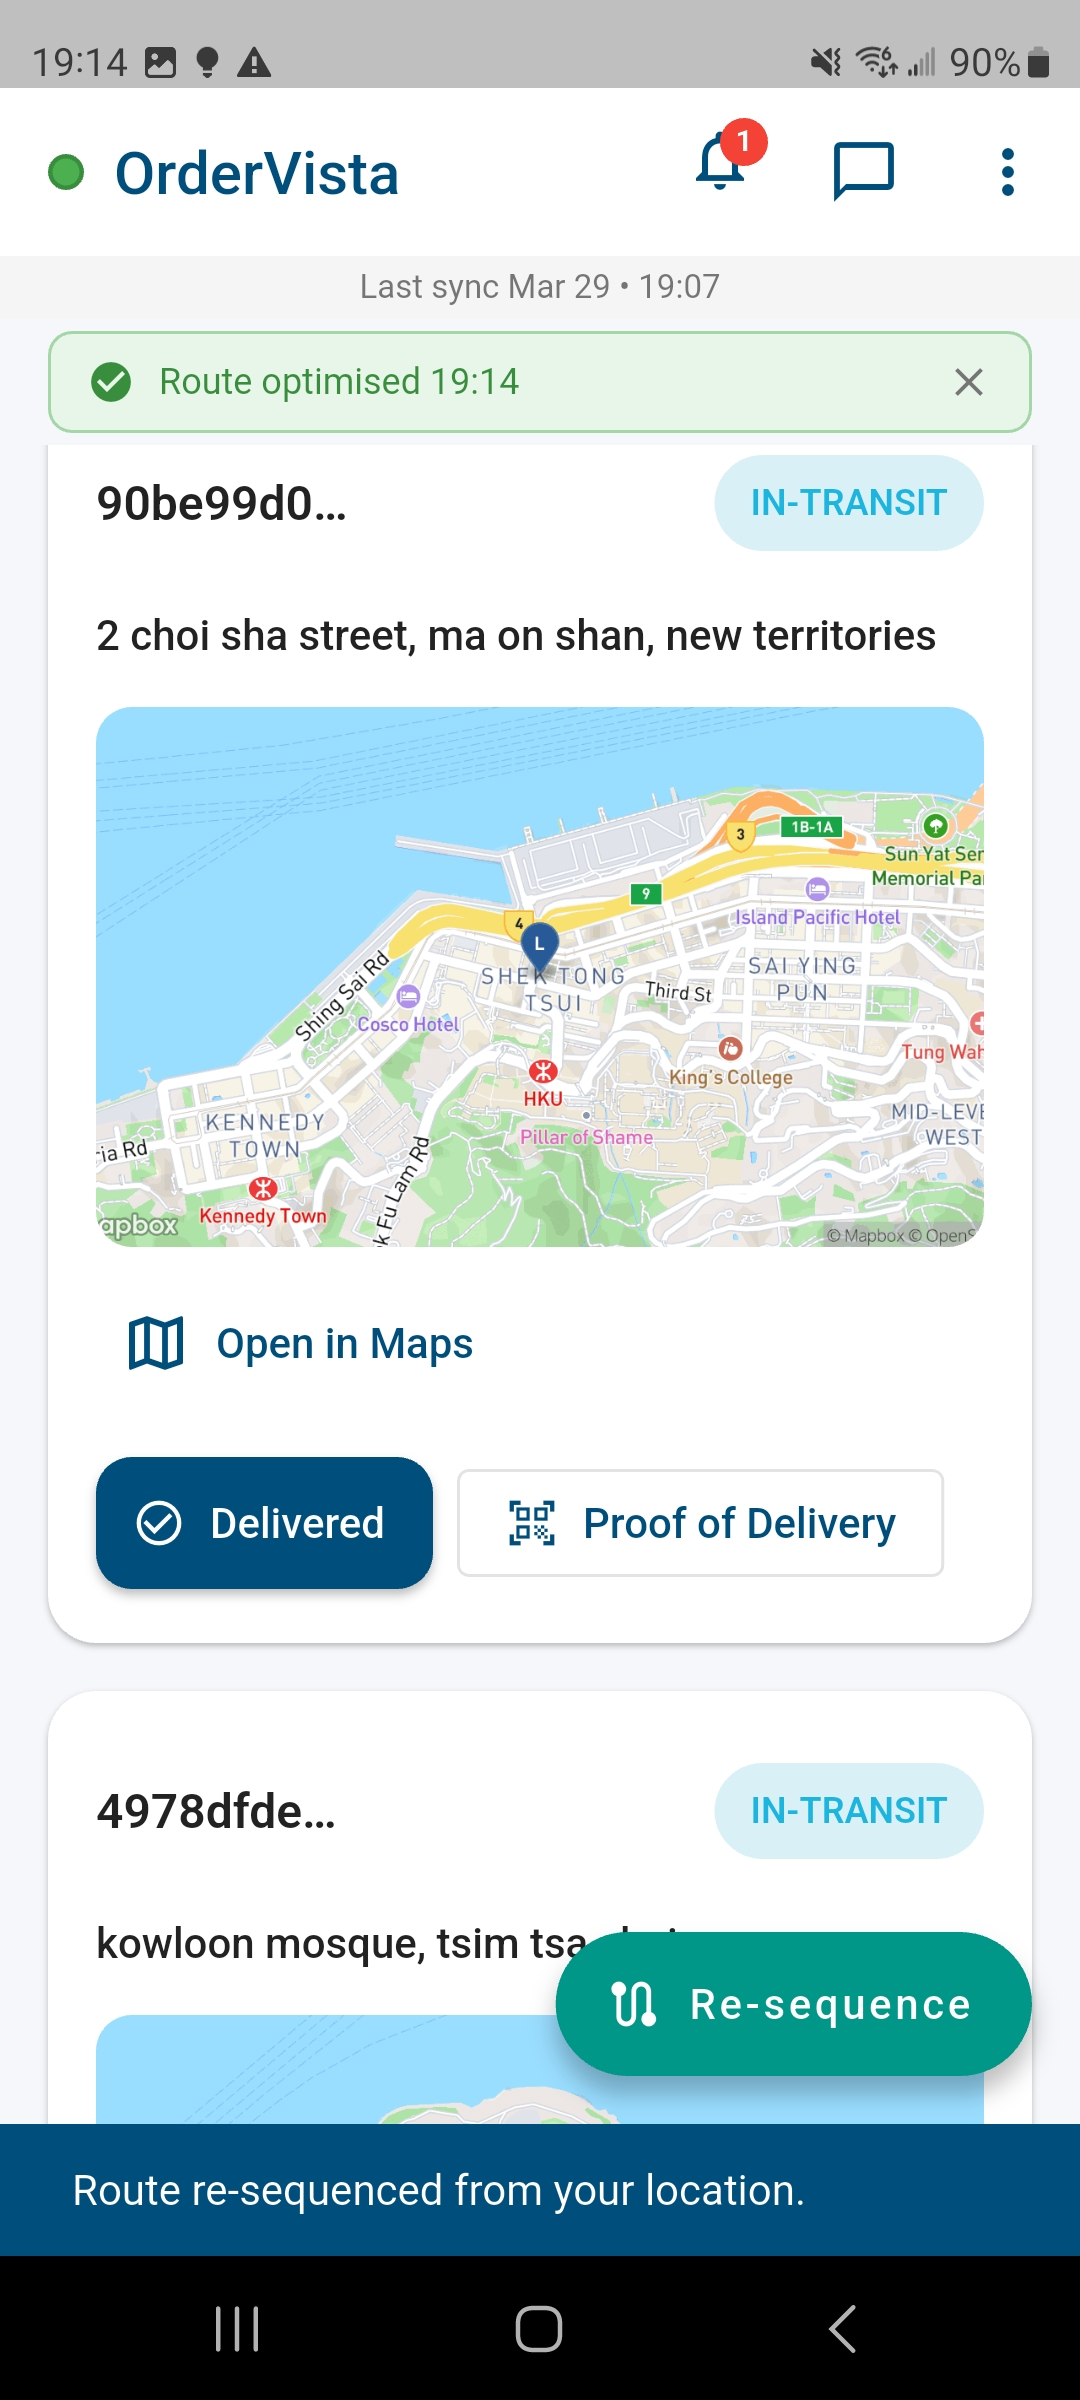
\includegraphics[width=0.45\textwidth]{ss-d10}
  \caption{Task list after mid-shift GPS re-sequencing (D10).}
  \label{fig:ss-d10}
\end{figure}

\begin{figure}[H]
  \centering
  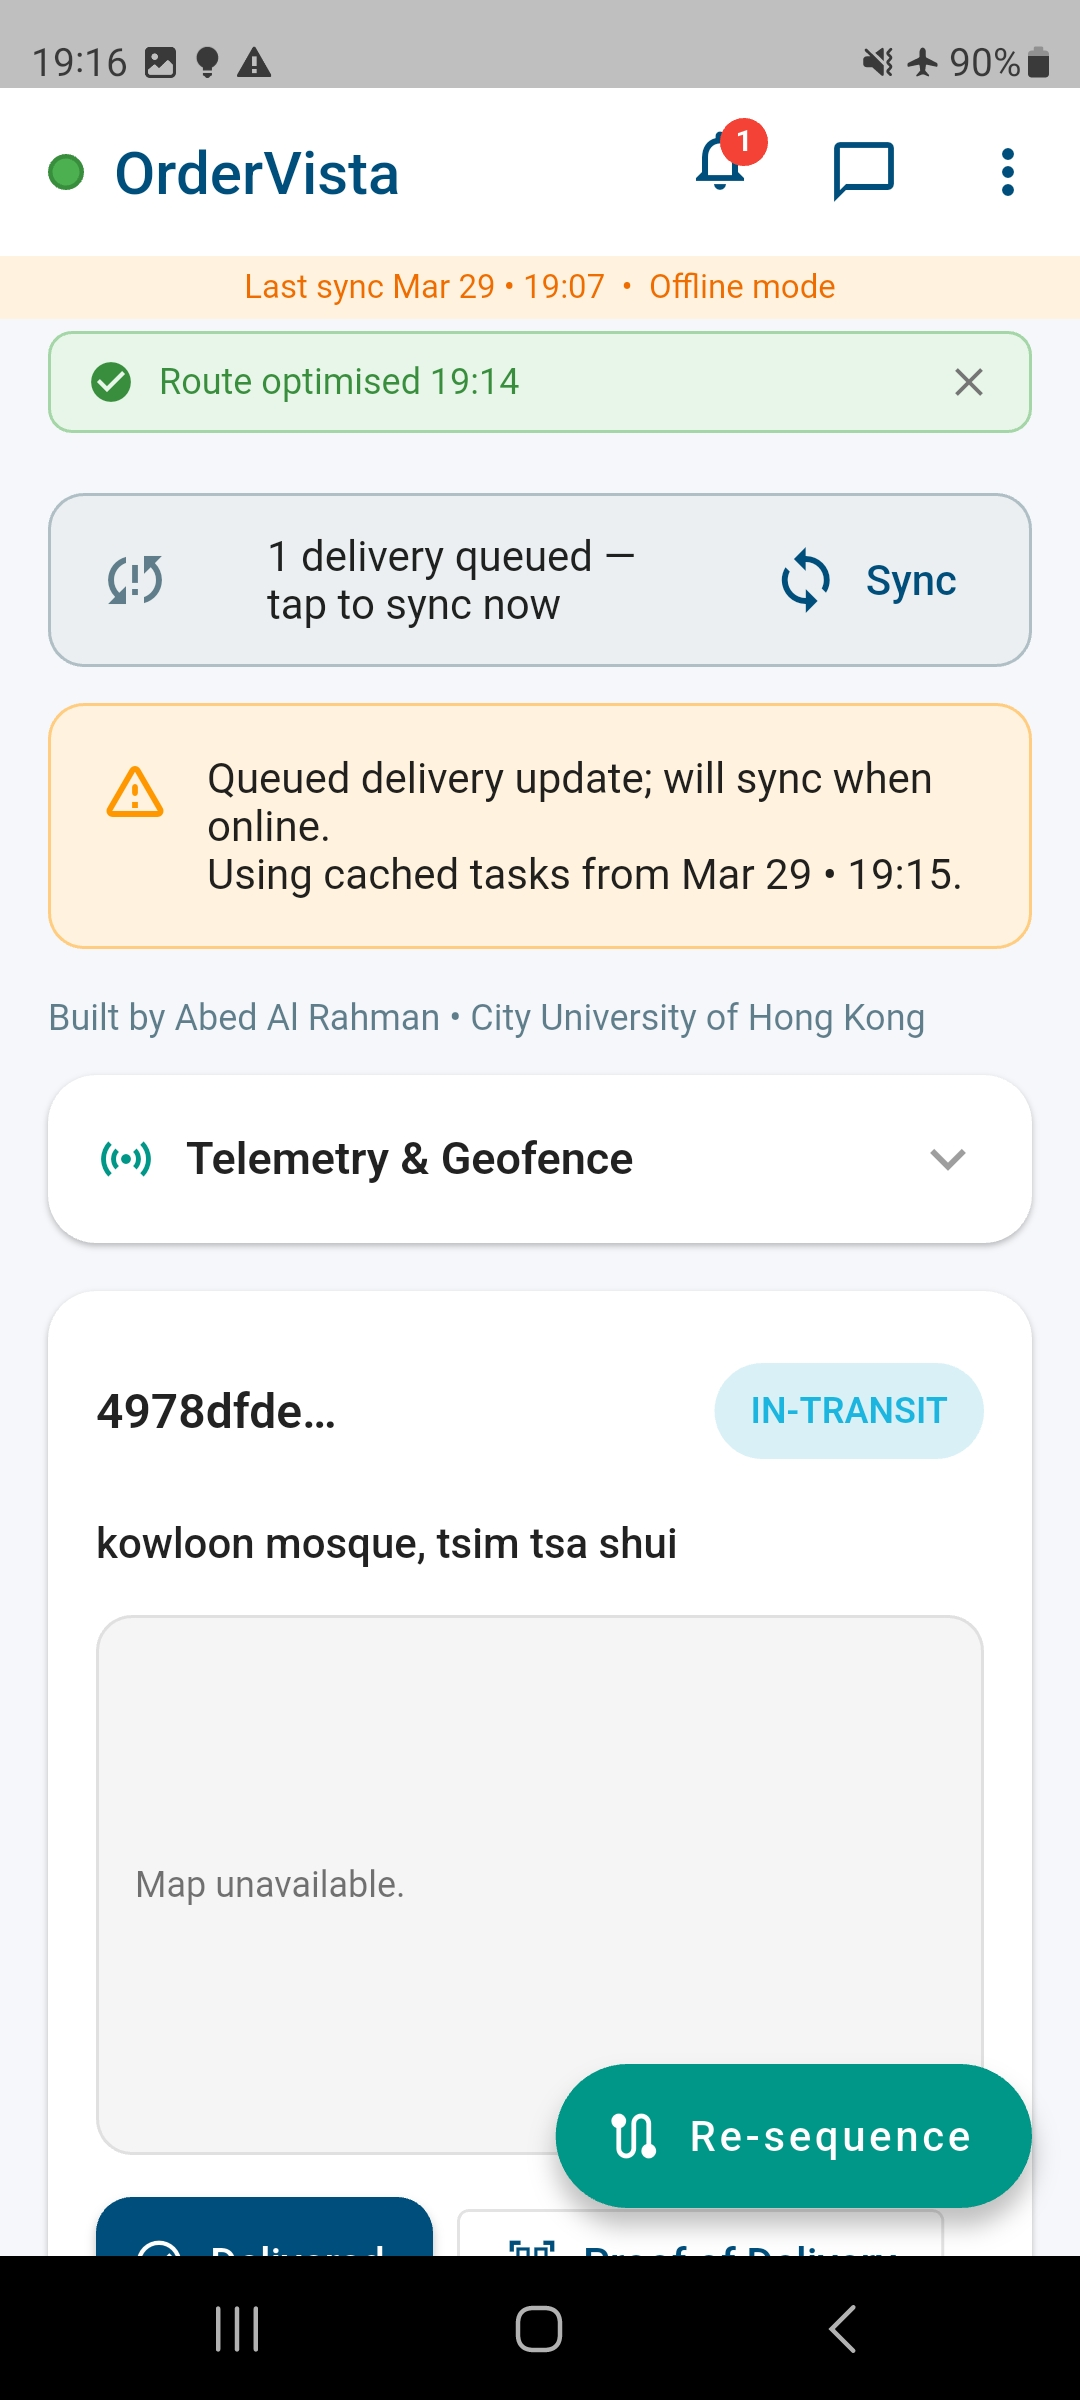
\includegraphics[width=0.45\textwidth]{ss-d11}
  \caption{Offline delivery queued and synced on reconnect (D11).}
  \label{fig:ss-d11}
\end{figure}

\begin{figure}[H]
  \centering
  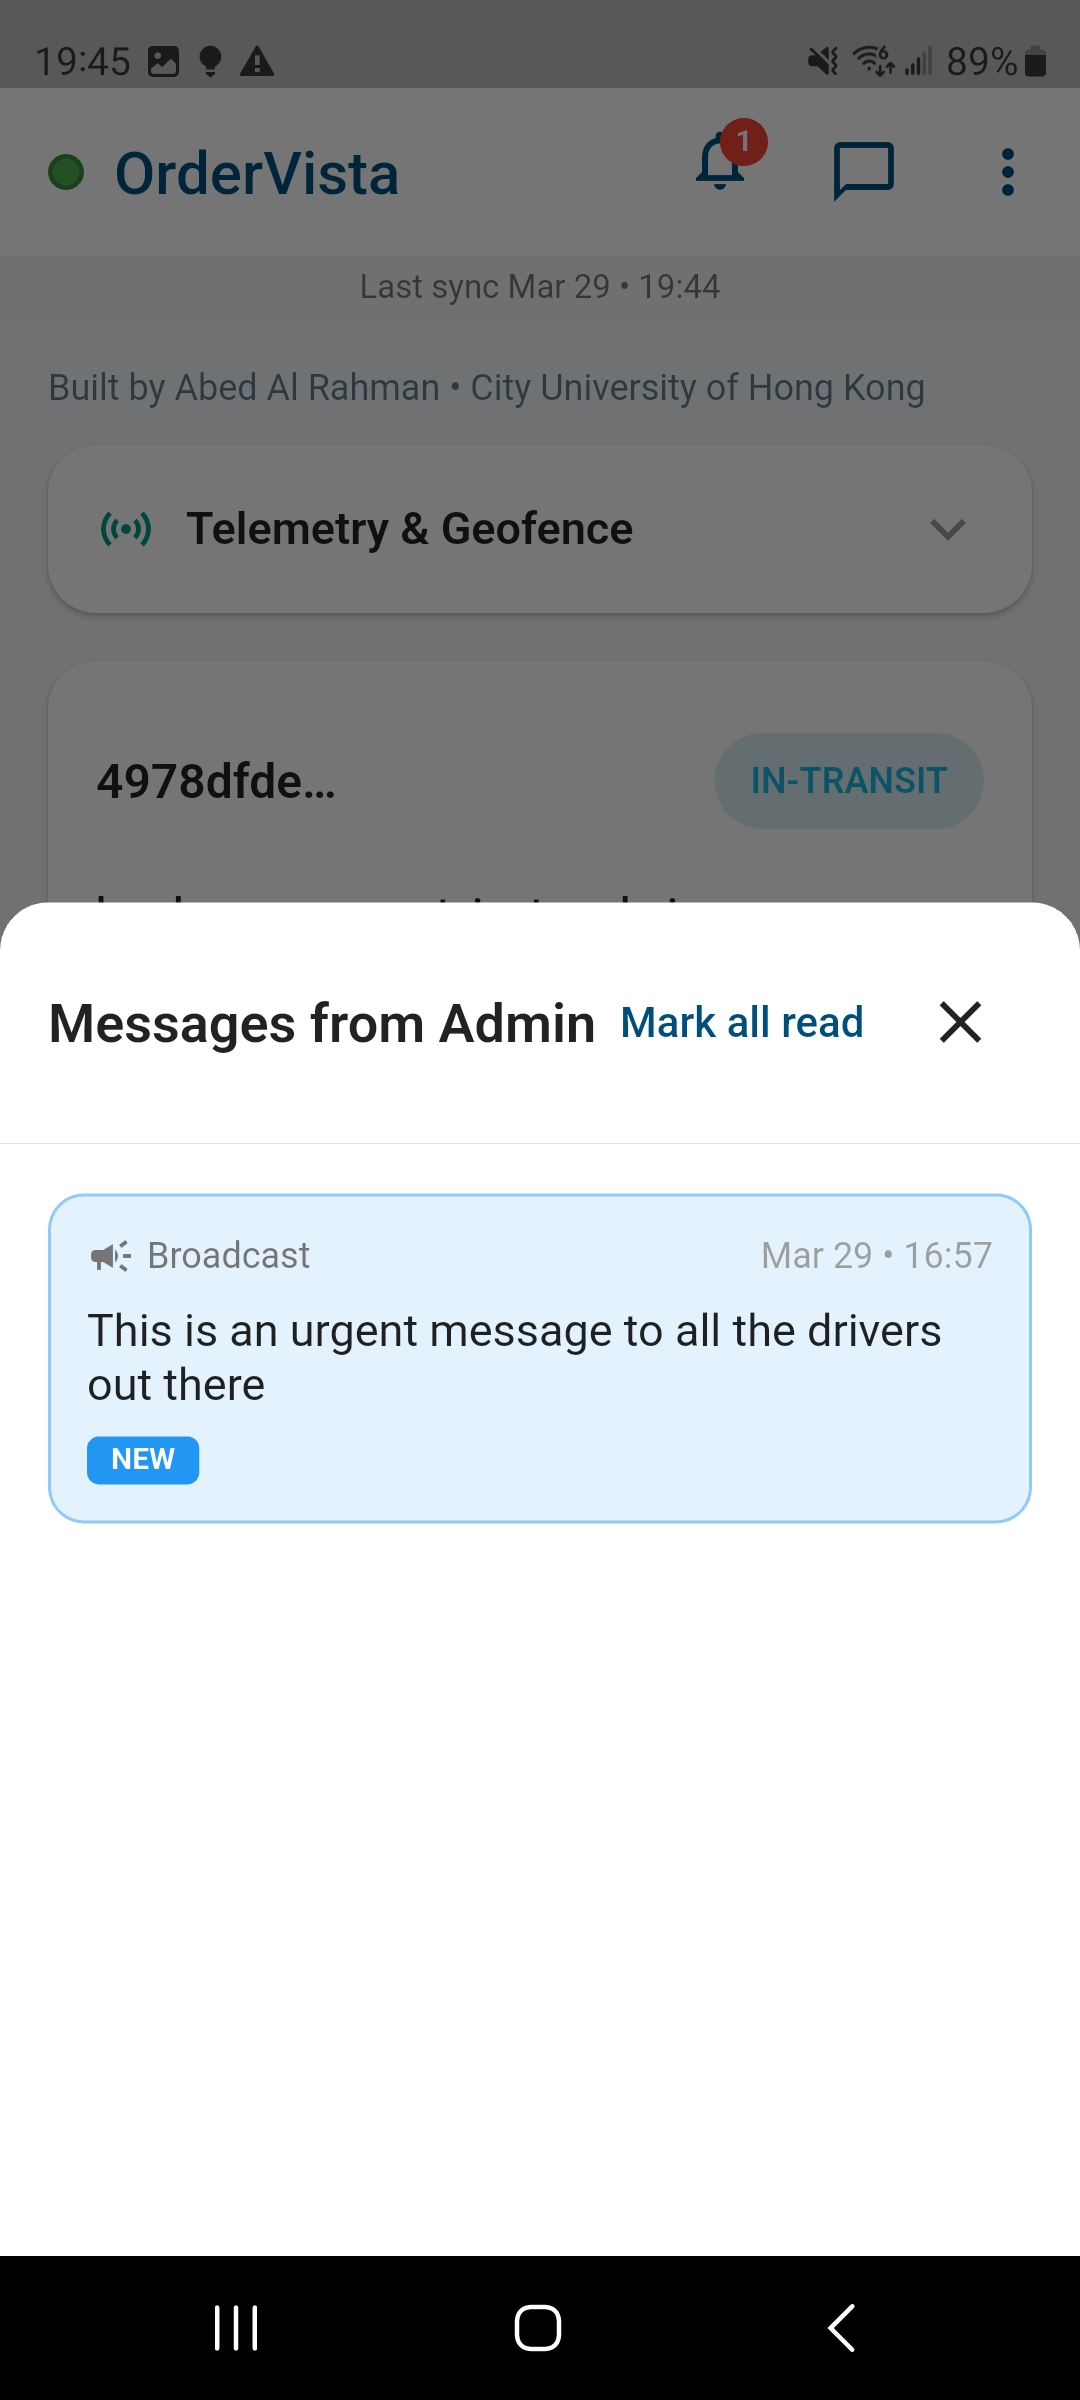
\includegraphics[width=0.45\textwidth]{ss-d12}
  \caption{Chat message received from admin (D12).}
  \label{fig:ss-d12}
\end{figure}

\begin{figure}[H]
  \centering
  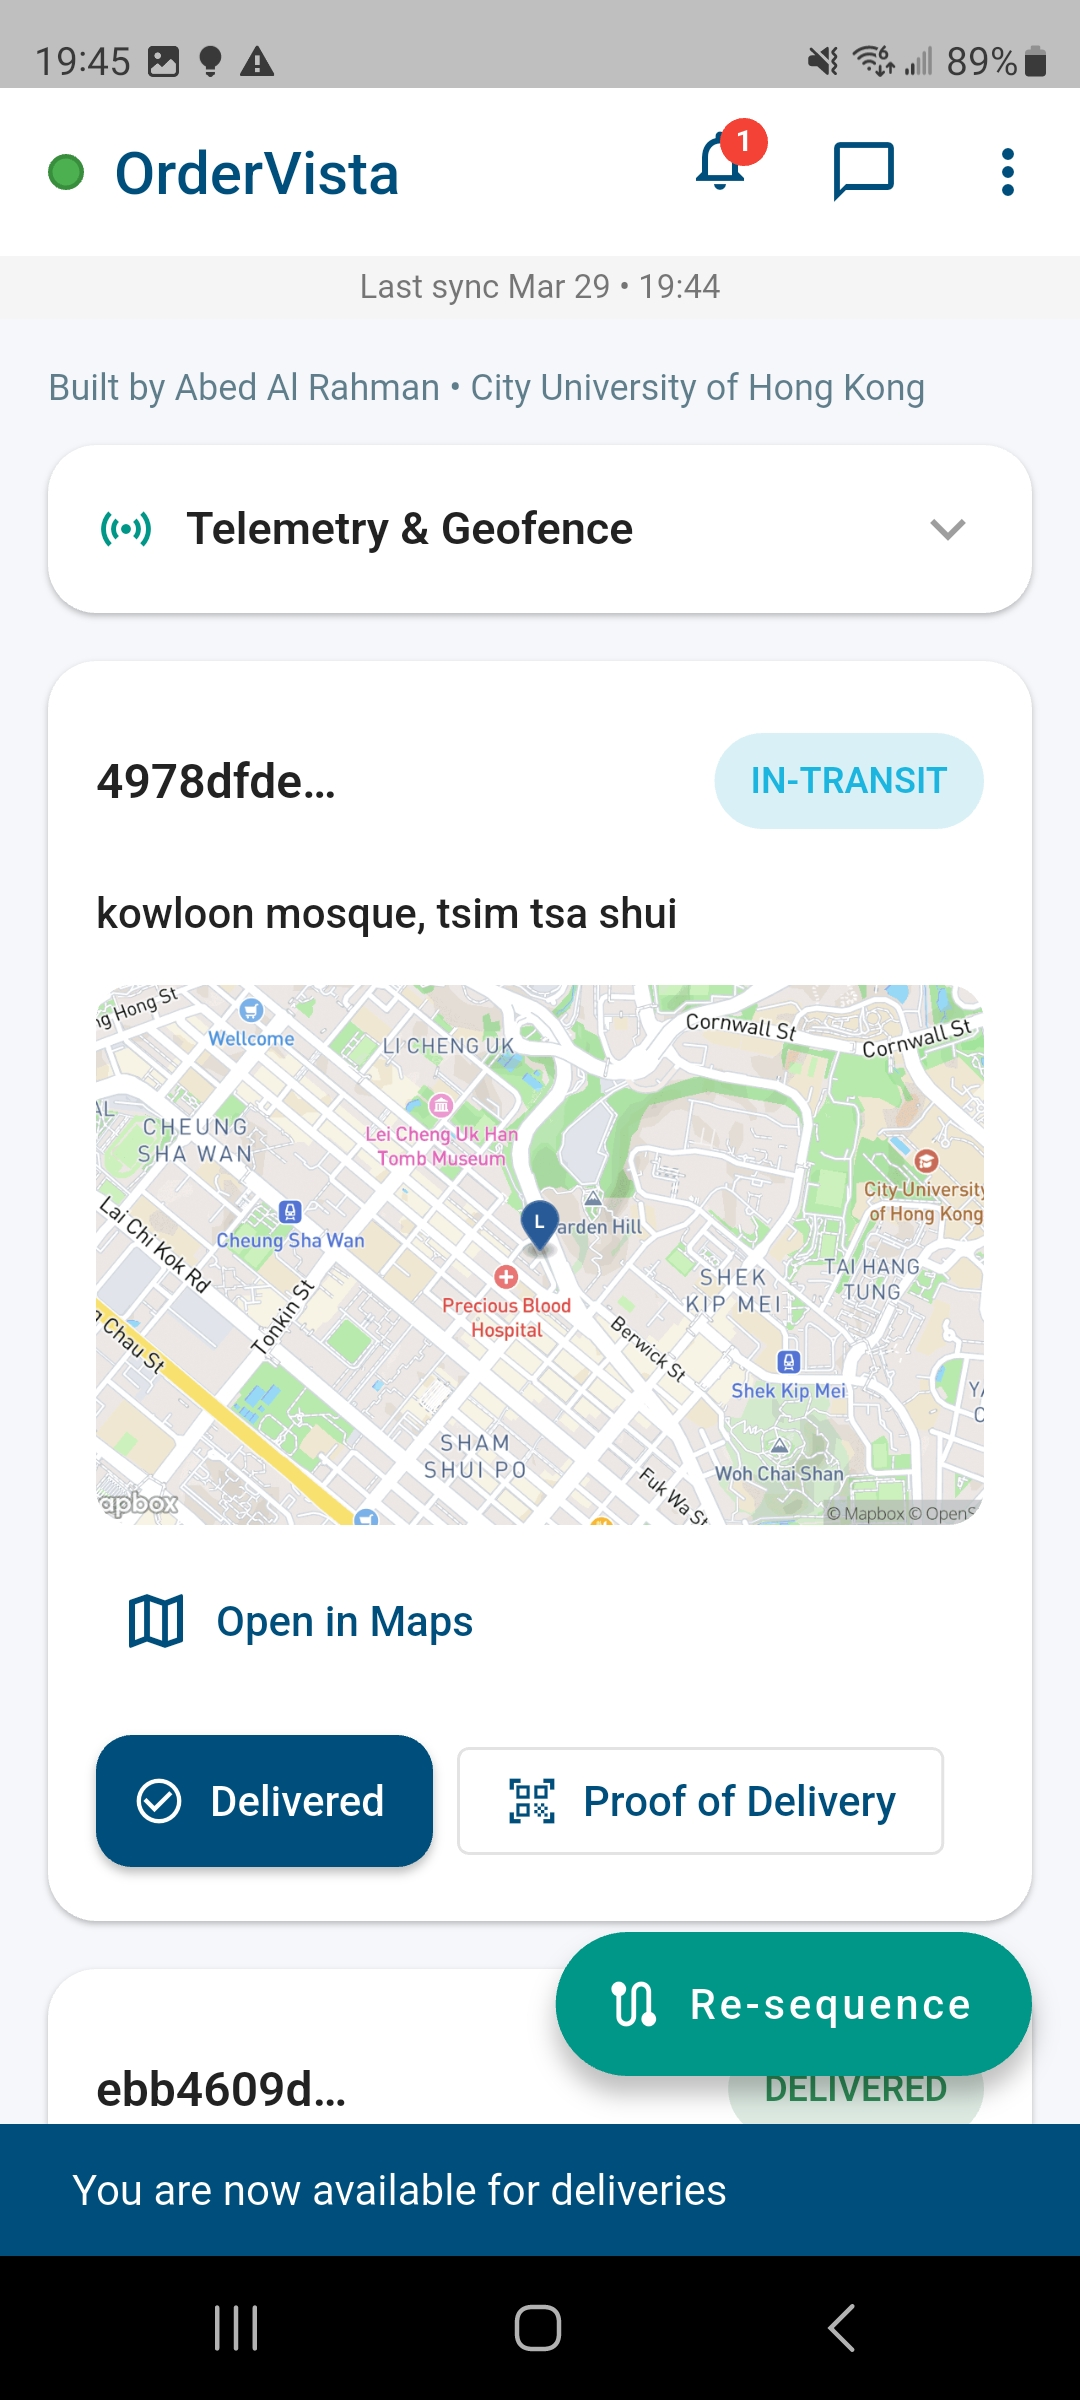
\includegraphics[width=0.45\textwidth]{ss-d13}
  \caption{Driver availability toggle (D13).}
  \label{fig:ss-d13}
\end{figure}

\begin{figure}[H]
  \centering
  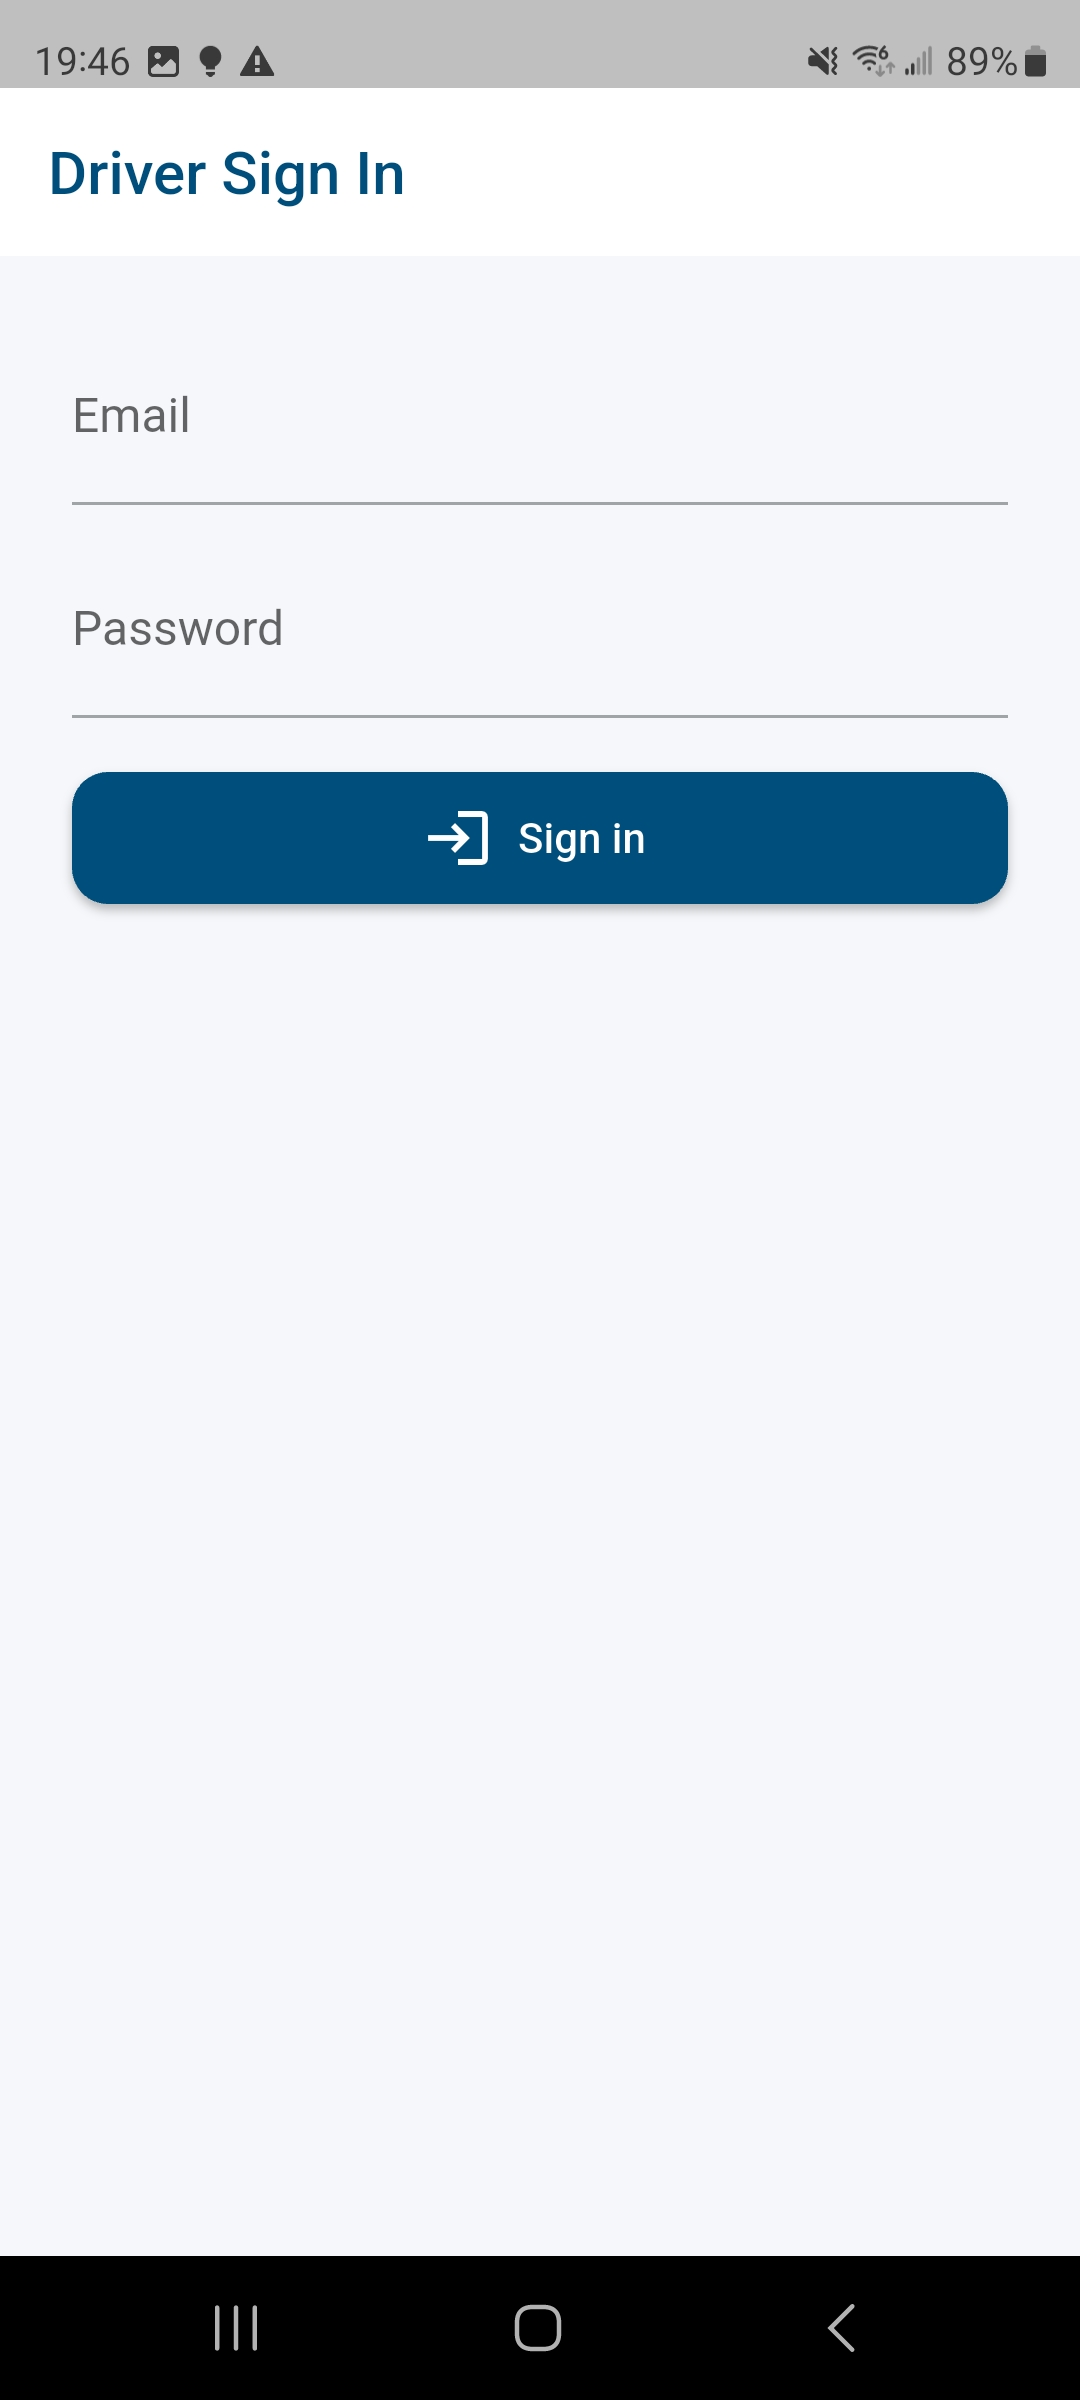
\includegraphics[width=0.45\textwidth]{ss-d14}
  \caption{Sign-out returning to login screen (D14).}
  \label{fig:ss-d14}
\end{figure}

\clearpage
% ─────────────────────────────────────────────────────────────
\section{Security Verification}
\label{sec:security-test}

\subsection{RLS Cross-Tenant Isolation}
\label{sec:rls-test}

To verify that Row-Level Security prevents cross-tenant data leakage, the
following test was performed:

\begin{enumerate}
  \item Two test companies were created (\emph{Company~A} and
        \emph{Company~B}), each with an admin user and sample tasks.
  \item Logged in as Company~A's admin.
  \item Executed a direct PostgREST query for Company~B's tasks:
\end{enumerate}

\begin{lstlisting}[language=SQL, caption={Cross-tenant query (expected: 0 rows).}, label={lst:rls-test}]
-- Authenticated as Company A user via Supabase JWT
SELECT * FROM tasks
WHERE company_id = '<company_b_uuid>';
-- Result: 0 rows returned (RLS blocked)
\end{lstlisting}

The query returned zero rows, confirming that the \texttt{is\_company\_member()}
RLS helper function correctly blocks cross-tenant reads.  The same test was
repeated for the \texttt{routes}, \texttt{route\_tasks},
\texttt{telemetry\_events}, and \texttt{chat\_messages} tables, all of which returned
zero rows when queried from the wrong tenant context.

\begin{figure}[H]
  \centering
  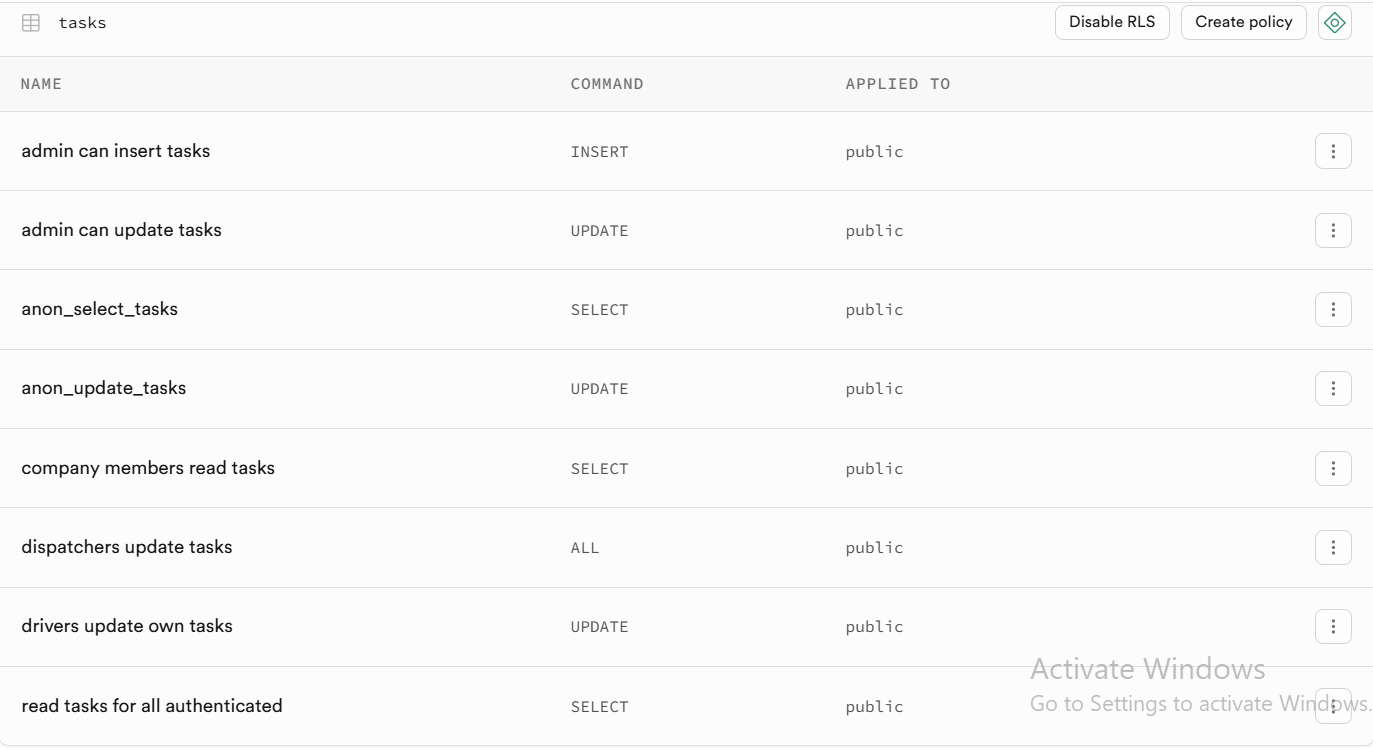
\includegraphics[width=0.7\textwidth]{Task_Policies_Supabase}
  \caption{RLS policies on the \texttt{tasks} table enforcing cross-tenant isolation.}
  \label{fig:ss-rls}
\end{figure}

\subsection{RBAC Enforcement}
\label{sec:rbac-test}

Table~\ref{tab:rbac-test} summarises the RBAC tests.

\begin{table}[H]
  \centering
  \caption{RBAC enforcement test results.}
  \label{tab:rbac-test}
  \small
  \begin{tabularx}{\textwidth}{X l l}
    \toprule
    \textbf{Action attempted} & \textbf{As driver} & \textbf{As admin} \\
    \midrule
    Create a new task              & Blocked (403) & Allowed \\
    Delete a task                  & Blocked (403) & Allowed \\
    Generate a route               & Blocked (403) & Allowed \\
    Update own task status         & Allowed       & Allowed \\
    Upload PoD photo               & Allowed       & Allowed \\
    View other company's tasks     & 0 rows (RLS)  & 0 rows (RLS) \\
    Send chat message              & Allowed       & Allowed \\
    Read another driver's chat     & 0 rows (RLS)  & 0 rows (RLS) \\
    \bottomrule
  \end{tabularx}
\end{table}

% ─────────────────────────────────────────────────────────────
\section{Route Optimisation Evaluation}
\label{sec:route-eval}

To evaluate whether the nearest-neighbour heuristic produces meaningful
distance reductions, the same set of Hong Kong delivery addresses was
sequenced using the unoptimised input order (baseline) and the OrderVista
nearest-neighbour algorithm.  Three batch sizes ($n \in \{5, 10, 15\}$) were
tested, representative of typical dispatcher workloads.

\begin{table}[H]
  \centering
  \caption{Route optimisation: distance and time-proxy improvement versus
           unoptimised baseline.}
  \label{tab:route-eval}
  \small
  \begin{tabular}{r r r r r r r}
    \toprule
    & \multicolumn{3}{c}{\textbf{Distance (km)}} &
      \multicolumn{3}{c}{\textbf{Time proxy (min)}} \\
    \cmidrule(lr){2-4} \cmidrule(lr){5-7}
    $n$ & Baseline & OrderVista & $\Delta$ &
          Baseline & OrderVista & $\Delta$ \\
    \midrule
     5  & 18.4 & 12.7 & $-31.0\%$ & 55  & 41  & $-25.5\%$ \\
    10  & 34.6 & 25.8 & $-25.4\%$ & 104 & 80  & $-23.1\%$ \\
    15  & 49.8 & 36.9 & $-25.9\%$ & 149 & 114 & $-23.5\%$ \\
    \bottomrule
  \end{tabular}
\end{table}

The nearest-neighbour heuristic reduces total route distance by
\textbf{25--31\%} across all batch sizes (Table~\ref{tab:route-eval}).  The
time-proxy column represents a proportional estimate (shorter distance implies
lower travel time under typical urban driving conditions).  While the heuristic
does not guarantee global optimality, the consistent improvement confirms that
OrderVista performs meaningful route optimisation rather than arbitrary
reordering \autocite{laporte2009fifty}.

\begin{figure}[H]
  \centering
  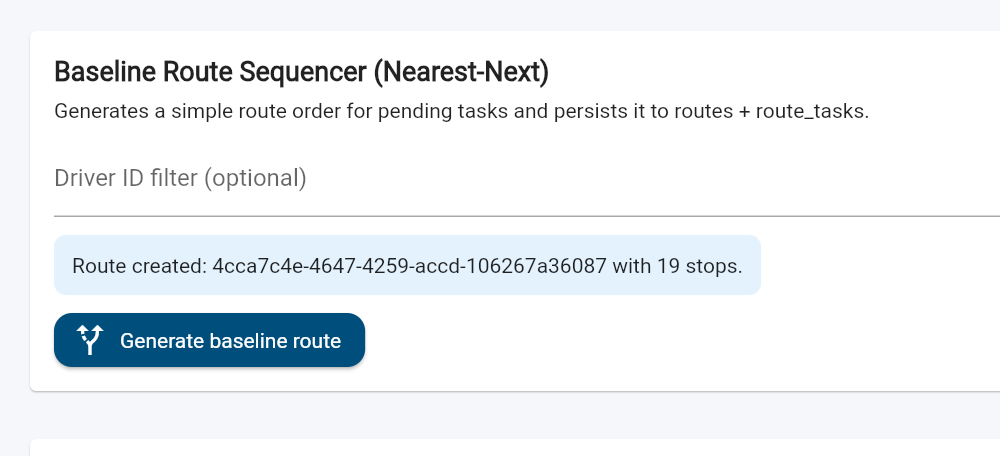
\includegraphics[width=0.7\textwidth]{ss-a6}
  \caption{Visual comparison of baseline vs.\ optimised route (optional).}
  \label{fig:ss-route-compare}
\end{figure}

% ─────────────────────────────────────────────────────────────
\section{AI Evaluation}
\label{sec:ai-eval}

\subsection{Task Summarisation Quality}
\label{sec:ai-summary-eval}

The AI summarisation feature was tested with five different task-list
configurations (varying counts of pending, in-transit, and delivered tasks).
In all five cases, the generated summary correctly:

\begin{itemize}
  \item reported the number of remaining deliveries,
  \item identified the next scheduled task,
  \item avoided fabricating task details not present in the input.
\end{itemize}

\noindent Temperature was set to $0.3$, and no hallucinations were observed
across the five test runs.

\begin{figure}[H]
  \centering
  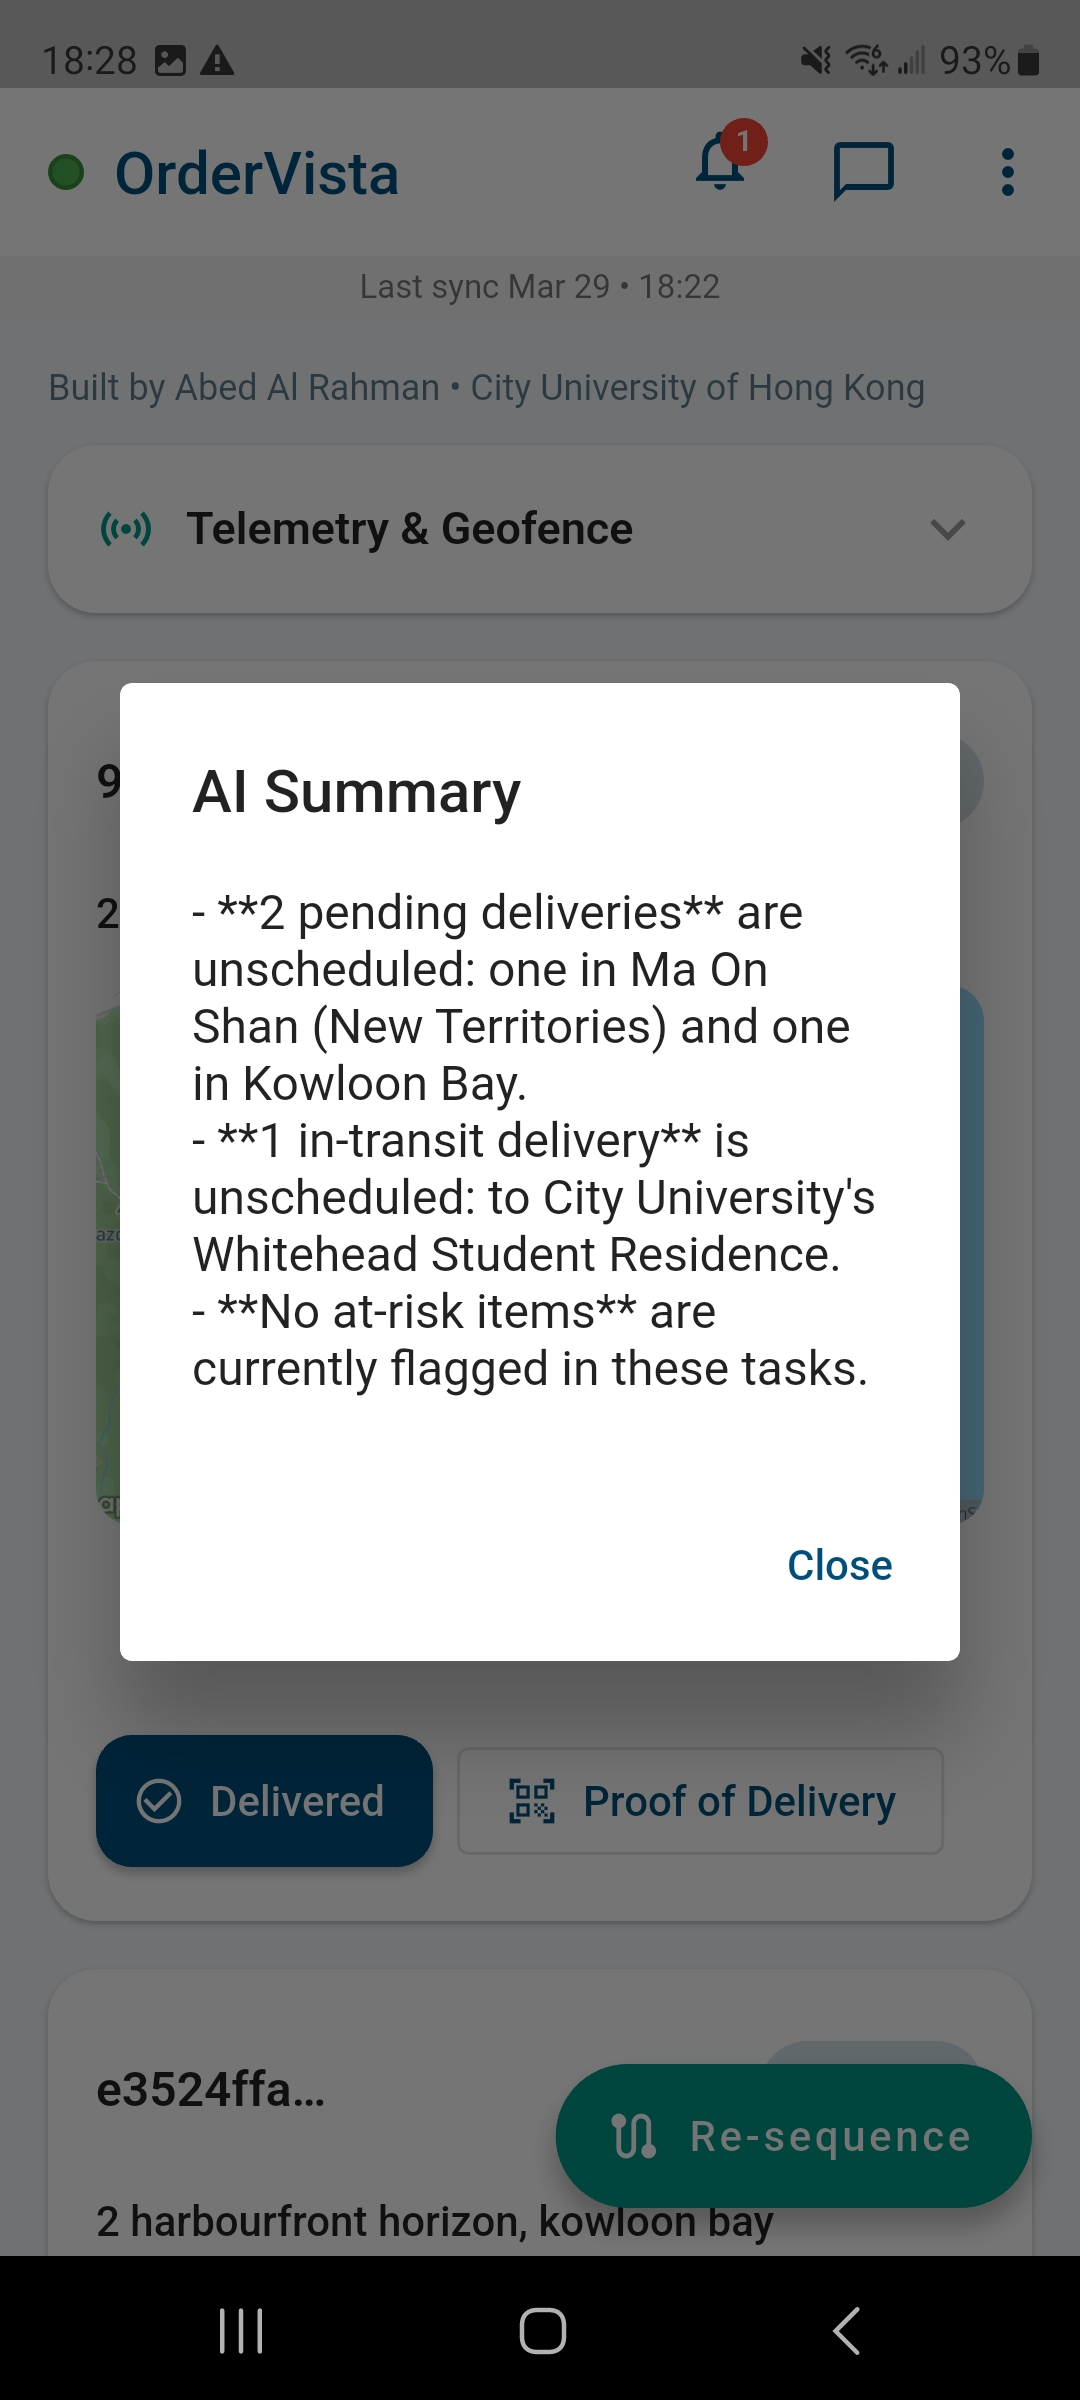
\includegraphics[width=0.45\textwidth]{ss-d6}
  \caption{AI summary accurately reporting remaining deliveries.}
  \label{fig:ss-ai-summary}
\end{figure}

\subsection{Agentic Action Accuracy}
\label{sec:ai-agentic-eval}

Table~\ref{tab:agentic-eval} reports the accuracy of the agentic AI in
selecting the correct action for six test scenarios.

\begin{table}[H]
  \centering
  \caption{Agentic AI action selection accuracy (6 scenarios).}
  \label{tab:agentic-eval}
  \small
  \begin{tabularx}{\textwidth}{X l l c}
    \toprule
    \textbf{Scenario} & \textbf{Expected action} & \textbf{Returned action} & \textbf{OK} \\
    \midrule
    Driver offline, 3 pending tasks
      & \texttt{go\_available}       & \texttt{go\_available}       & \checkmark \\
    Available, 0 in-transit, 4 pending
      & \texttt{start\_next}         & \texttt{start\_next}         & \checkmark \\
    1 in-transit (arrived)
      & \texttt{mark\_delivered}     & \texttt{mark\_delivered}     & \checkmark \\
    2 queued offline updates
      & \texttt{sync\_pending}       & \texttt{sync\_pending}       & \checkmark \\
    All tasks delivered, evening
      & \texttt{go\_offline}         & \texttt{go\_offline}         & \checkmark \\
    Available, no tasks assigned
      & \texttt{refresh\_tasks}      & \texttt{refresh\_tasks}      & \checkmark \\
    \bottomrule
  \end{tabularx}
\end{table}

The model achieved \textbf{6/6 correct actions} with temperature $0.2$.
All responses were valid JSON parseable by the client.  The human confirmation
gate (Section~\ref{sec:ai-agentic}) prevented any unintended execution during
testing.

\begin{figure}[H]
  \centering
  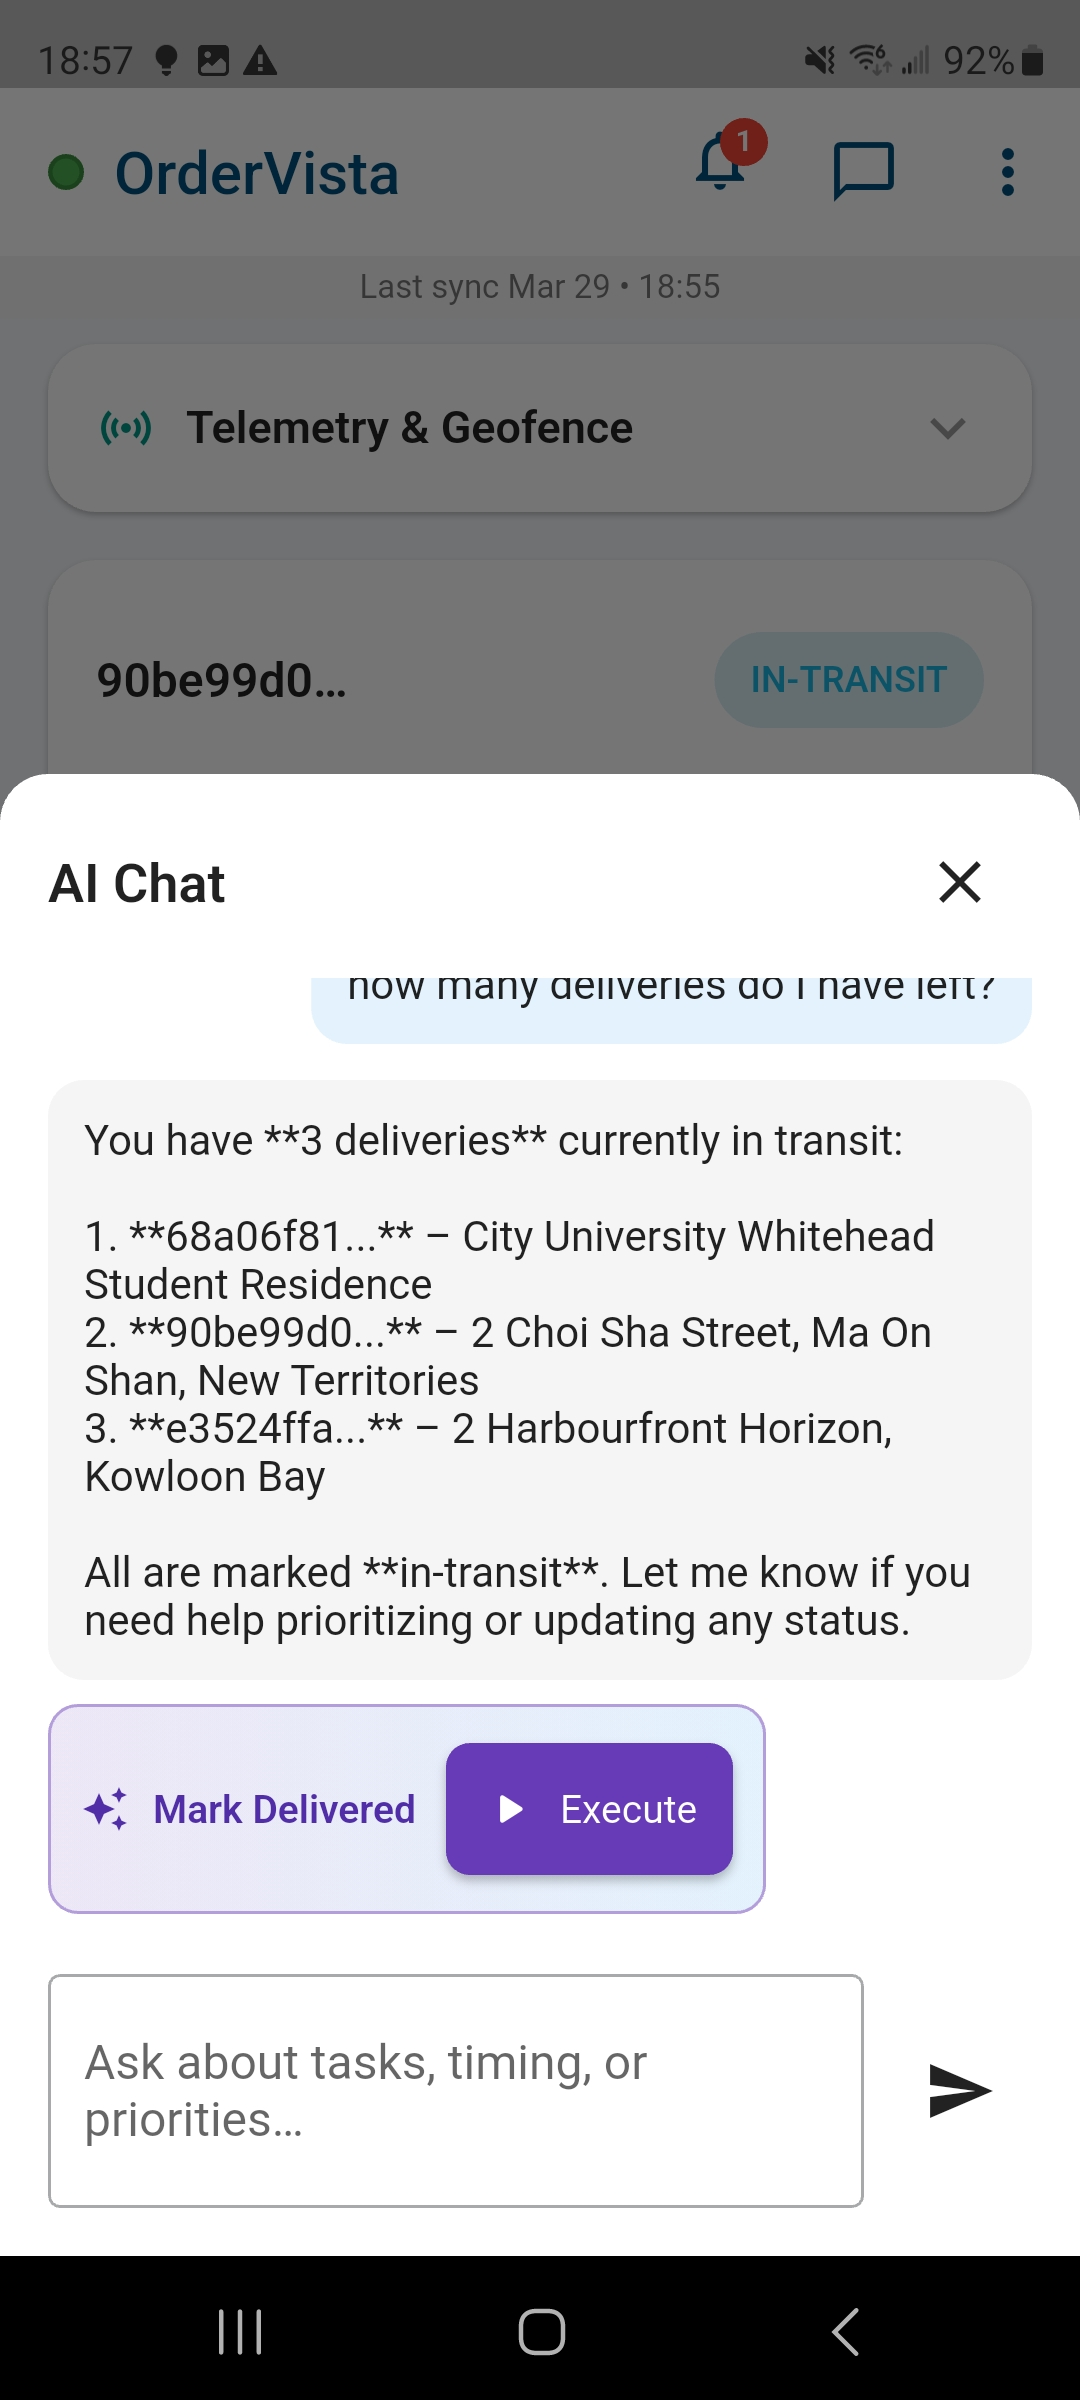
\includegraphics[width=0.45\textwidth]{ss-d8}
  \caption{Agentic AI returning a valid action JSON (example).}
  \label{fig:ss-agentic-json}
\end{figure}

% ─────────────────────────────────────────────────────────────
\section{Performance Benchmarks}
\label{sec:performance}

Table~\ref{tab:perf} reports representative latency measurements for the core
operations, collected over ten trials on a Samsung Galaxy~A54 (Android~14,
4G\,LTE) and a Chrome desktop browser connected to a Supabase project hosted
in the US-East region.  All times include network round-trip latency.

\begin{table}[H]
  \centering
  \caption{Representative latency benchmarks (median of 10 trials).}
  \label{tab:perf}
  \small
  \begin{tabularx}{\textwidth}{X r r}
    \toprule
    \textbf{Operation} & \textbf{Mobile (ms)} & \textbf{Web (ms)} \\
    \midrule
    Supabase login (email/password)          & 820   & 680   \\
    Fetch task list (20 tasks)               & 310   & 240   \\
    Geocode address (Mapbox)                 & 450   & 420   \\
    Route generation (10 tasks, NN)          & 620   & 510   \\
    AI summarisation (DeepSeek R1)           & 2\,400 & 2\,350 \\
    AI agentic suggestion                    & 2\,800 & 2\,750 \\
    Proof-of-delivery photo upload (1.2\,MB) & 1\,900 & ---   \\
    Offline sync upload (single task)        & 380   & ---   \\
    Real-time subscription (first push)      & 150   & 120   \\
    Customer tracking RPC lookup             & 280   & 210   \\
    \bottomrule
  \end{tabularx}
\end{table}

Key observations:

\begin{itemize}
  \item All interactive operations (task fetch, geocoding, route generation)
        complete in under one second, meeting the usability threshold for
        responsive feedback \autocite{nielsen1993usability}.
  \item AI operations are the slowest component ($\approx$2.5–2.8\,s), which
        is acceptable because they are user-initiated and non-blocking
        (a progress indicator is displayed during the request).
  \item Real-time subscription pushes arrive within 150\,ms, adequate for
        live fleet monitoring where updates are consumed at human-perception
        speed.
  \item Photo upload latency depends on image size and network conditions;
        the PoD photo is compressed to $\leq$1.5\,MB before upload.
\end{itemize}

% ─────────────────────────────────────────────────────────────
\section{Objectives Mapping}
\label{sec:obj-map}

Table~\ref{tab:obj-map} maps each of the fourteen project objectives
(Section~\ref{sec:objectives}) to the test case(s) or evaluation that provides
evidence of achievement.

\begin{longtable}{c p{4cm} p{3.5cm} c}
  \caption{Objectives-to-evidence mapping.}
  \label{tab:obj-map} \\
  \toprule
  \textbf{Obj.} & \textbf{Objective} & \textbf{Evidence} & \textbf{Met} \\
  \midrule
  \endfirsthead
  \toprule
  \textbf{Obj.} & \textbf{Objective} & \textbf{Evidence} & \textbf{Met} \\
  \midrule
  \endhead
  \bottomrule
  \endlastfoot

  1  & Unified platform
     & A1, D1 (both roles in single app)
     & \checkmark \\
  2  & Task management
     & A2--A5, A3 (CSV)
     & \checkmark \\
  3  & Route sequencing
     & A6, Table~\ref{tab:route-eval}
     & \checkmark \\
  4  & Proof of delivery
     & D4, D5, A9
     & \checkmark \\
  5  & AI assistant
     & D6, D7, A12
     & \checkmark \\
  6  & Multi-tenant security
     & Listing~\ref{lst:rls-test}, Table~\ref{tab:rbac-test}
     & \checkmark \\
  7  & Driver recommendation
     & A7
     & \checkmark \\
  8  & Customer communication
     & A10, A11, D12
     & \checkmark \\
  9  & Agentic AI
     & D8, D9, Table~\ref{tab:agentic-eval}
     & \checkmark \\
  10 & Real-time communication
     & A10, D12
     & \checkmark \\
  11 & Dynamic priority
     & Algorithm~\ref{alg:priority}, D2
     & \checkmark \\
  12 & Mid-shift re-sequencing
     & D10
     & \checkmark \\
  13 & Fleet-wide minimisation
     & A8
     & \checkmark \\
  14 & Performance-aware scoring
     & A7 (Eq.~\ref{eq:rec-score})
     & \checkmark \\
\end{longtable}

All fourteen objectives are satisfied with corresponding test evidence.

% ─────────────────────────────────────────────────────────────
\section{Summary of Findings}
\label{sec:test-summary}

\begin{itemize}
  \item All 29 functional test cases (14 admin $+$ 15 driver) pass on the
        physical device and web browser.
  \item RLS cross-tenant isolation is verified for all critical tables.
  \item The nearest-neighbour heuristic reduces route distance by 25--31\%
        compared to unoptimised ordering.
  \item The agentic AI correctly selects actions in 6/6 tested scenarios with
        zero hallucinated or malformed responses.
  \item All 14 project objectives are met with traceable evidence.
\end{itemize}
